\documentclass[a4paper,11pt]{article}
% \pdfoutput=1 % if your are submitting a pdflatex (i.e. if you have
             % images in pdf, png or jpg format)
\usepackage{jcappub} % for details on the use of the package, please
                     % see the JCAP-author-manual
\usepackage[T1]{fontenc} % if needed
\usepackage{float} 
\usepackage{lmodern}
\usepackage{booktabs}
\usepackage{siunitx}
\usepackage[english]{babel}
\addto\captionsenglish{
  \renewcommand{\figurename}{Figure}
  \renewcommand{\tablename}{Table}
}
\usepackage[utf8]{inputenc}
\usepackage{natbib}
\usepackage[colorlinks=true, citecolor=blue, urlcolor=blue, linkcolor=blue]{hyperref} 
\usepackage{graphicx}
\usepackage{subfigure}% Include figure files
\usepackage[justification=raggedright]{caption}
\usepackage{tabularx}
\usepackage{dcolumn}% Align table columns on decimal point
\usepackage{bm}
% \usepackage{ulem}

\newcommand{\ms}{M_\odot}
\newcommand{\bmt}{{\bm{\theta}}}
\newcommand{\bmT}{{\bm{\Theta}}}
\newcommand{\bmH}{{\bm{H}}}
\newcommand{\rmd}{{\rm{d}}}
\newcommand{\ZW}[1]{\textcolor{magenta}{$\mathcal{ZW}$:~#1}}

% \newcommand{\DL}[1]{\textcolor{red}{#1}} 
% \newcommand{\LS}[1]{\textcolor{cyan}{\bf #1}} 
% \newcommand{\YG}[1]{\textcolor{blue}{#1}} 
% \newcommand{\ZW}[2]{{\color{blue} \sout{#1} ZW: {#2}}} % For comment
% \newcommand{\Reply}[1]{{\bf\color{blue} #1}}

\title{Inference of Love-Q relations with gravitational waves in hierarchical Bayesian framework}

%% %simple case: 2 authors, same institution
%% \author{A. Uthor}
%% \author{and A. Nother Author}
%% \affiliation{Institution,\\Address, Country}

% more complex case: 4 authors, 3 institutions, 2 footnotes
\author[a]{Zhihao Zheng,}
\author[b,c,1]{Ziming Wang\note{Corresponding author.},}
\author[d]{Jinwen Deng,}
\author[b,c]{Yiming Dong,}
\author[c,e,1]{and Lijing Shao}


% The "\note" macro will give a warning: "Ignoring empty anchor..."
% you can safely ignore it.

\affiliation[a]{School of Yuanpei, Peking University,
Beijing 100871, China}
\affiliation[b]{Department of Astronomy, School of Physics, Peking University,
Beijing 100871, China}
\affiliation[c]{Kavli Institute for Astronomy and Astrophysics, Peking
University, Beijing 100871, China}
\affiliation[d]{School of Physics, Peking University,
Beijing 100871, China}
\affiliation[e]{National Astronomical Observatories, Chinese Academy of
Sciences, Beijing 100012, China}

% \affiliation[a]{One University,\\some-street, Country}
% \affiliation[b]{Another University,\\different-address, Country}
% \affiliation[c]{A School for Advanced Studies,\\some-location, Country}

% e-mail addresses: one for each author, in the same order as the authors
\emailAdd{2300017794@stu.pku.edu.cn}
\emailAdd{zwang@pku.edu.cn}
\emailAdd{2300011335@stu.pku.edu.cn}
\emailAdd{ydong@pku.edu.cn}
\emailAdd{lshao@pku.edu.cn}

\abstract{Nuclear and gravity theories have predicted a universal ``Love-Q'' relation between the dimensionless tidal deformability $\Lambda$ and the dimensionless quadrupole moment $Q$ of neutron stars. However, this Love-Q relation has not yet been directly measured in an observational aspect. Gravitational waves (GWs) emitted from binary neutron star (BNS) systems serve as a powerful tool for probing NS properties and in the future, the next-generation GW detectors are expected to yield numerous BNS events with high-precision measurement. In this study, we explore the prospect of constraining the Love-Q relation with future GW observations. Adopting a hierarchical Bayesian framework, we are able to combine multiple GW events in a more systematic and robust manner. We simulate 1000 GW sources and select the loudest 20 of them for the analysis. We find that compared with the full quartic polynomial model, a linear relation between $\ln\Lambda$ and $\ln Q$ is accurate enough. We also discuss a quadratic and cubic polynomial Love-Q relations and find correlations between the parameters characterizing the Love-Q relation from linear to quartic polynomial models. Furthermore, we investigate the potential of the inferred Love-Q relation in testing modified gravity. Taking the dynamical Chern-Simons gravity as an example, our results suggest that the characteristic length can be limited to $\xi_{CS}^{1/4} \lesssim \mathcal{O}(10^1)$km with future GW observations. 
}

\begin{document}
\maketitle
\flushbottom

%=============================
\section{Introduction}
\label{sec:introducion}
%=============================

Neutron stars (NSs) serve as natural laboratories for studying nuclear and gravitational physics due to their extreme densities and strong gravitational fields. Electromagnetic observations of NSs, such as their observed maximum mass~\cite{Ozel:2010bz,Hebeler:2013nza,Antoniadis:2013pzd} and mass-radius relation~\cite{Lattimer:2006xb,Steiner:2010fz,Ozel:2010fw,Özel_2013,Guver:2013xa}, allow us to probe the properties of nuclear matter at densities exceeding nuclear saturation density. Besides, the recent observation of GW170817 has opened up a new observational window for investigating NS properties using gravitational waves (GWs) emitted during binary neutron star (BNS) 
coalescences~\cite{LIGOScientific:2017vwq,LIGOScientific:2018cki,LIGOScientific:2018hze}. Some of NS properties, including tidal deformability and spin-induced quadrupole moment, enter the GW waveform~\cite{Poisson:1997ha,Vines:2011ud,Favata:2013rwa,Wade:2014vqa,Samajdar:2019ulq,Abac:2023ujg} and therefore can be extracted from GW signals through parameter estimation~\cite{Harry:2018hke,Baiotti:2019sew,Chatziioannou:2020pqz,Agathos:2015uaa,Krishnendu:2017shb,Krishnendu:2019tjp,Lyu:2023zxv}. 

In a BNS system, tidal deformation occurs to each star due to the gravitational field of its companion~\cite{Hinderer:2007mb,Damour:2009vw}. The effect is characterized by the tidal deformability $\Lambda=2k_2/(3C^5)$, where $k_2$ is the tidal Love number and $C$ is the NS compactness~\cite{Flanagan:2007ix}. Also, a rotating NS experiences another deformation due to its spin, which induces a quadrupole moment $\mathcal{Q}=-Q\chi^2 m^3$ (spin-induced quadrupole moment, SIQM), where $Q$ is the dimensionless quadrupole moment,\footnote{We only talk about the dimensionless quadrupole moment later in the text. For simplicity, we call $Q$ ``the quadrupole moment'' without causing ambiguity.} $\chi$ is the NS dimensionless spin and $m$ is the NS mass~\cite{Hartle:1968,Laarakkers:1997hb}. Both $\Lambda$ and $Q$ can be calculated from $m$ with a fixed equation of state (EOS)~\cite{Yagi:2013awa}, which determine the pressure ($p$) as a function of density ($\rho$). 

Current observations have not yet confidently determined the actual EOS, but Yagi and Yunes~\cite{Yagi:2013bca,Yagi:2013awa} proposed a universal relation between $\Lambda$ (or tidal Love number) and $Q$. This Love-Q relation is EOS-insensitive with variation of about $1\%$ or less for different EOSs yet they can be dependent on the underlying gravity theory. Hence, measuring Love-Q relation allows for tests of gravity theories avoiding the interference from the uncertainty of EOS~\cite{Yagi:2013bca,Silva:2020acr,Shao:2022koz}. Previous works also adopted Love-Q relation to infer $Q$ from $\Lambda$ and to better estimate the spin parameters of BNSs~\cite{Yagi:2013bca,LIGOScientific:2018cki,LIGOScientific:2018hze,LIGOScientific:2020aai} with current GW detectors. 

Future next-generation ground based GW detectors, including the Cosmic Explorer (CE)~\cite{Reitze:2019iox,Reitze:2019dyk} and the Einstein Telescope (ET)~\cite{Punturo:2010zz,Hild:2010id,Sathyaprakash:2012jk}, will detect much more GW signals up to about $10^5$--$10^6$ events per year~\cite{LIGOScientific:2017zlf,Sathyaprakash:2019yqt,Kalogera:2021bya,Samajdar:2021egv}, thanks to their increased sensitivity and lower cutoff frequencies. These high-precision GW observations allow us to directly measure $\Lambda$ and $Q$ from BNS events and further infer the Love-Q relation. Samajdar and Dietrich~\cite{Samajdar:2020xrd} have first performed an analysis discussing the prospect of constraining Love-Q relation with GW observations, where they adopt a weighted linear regression. This treatment might miss the degeneracies and non-Gaussianality in the posterior of $\Lambda$ and $Q$. 

In this work, we adopt a hierarchical Bayesian framework combining multiple GW events to infer Love-Q relation with next-generation GW detector network. This framework has been applied in population property studies and EOS constraints~\cite{Mandel:2009nx,Mandel:2009pc,Adams:2012qw,Lackey:2014fwa,Mandel:2018mve,Thrane_2019,KAGRA:2021duu,Wang:2024xon}. Regarding the Love-Q relation parameters as hyperparameters, the hierarchical Bayesian framework separates the inferences of these hyperparameters and the single-event parameters into two levels. The framework is also able to deal with highly degenerate and non-Gaussian posteriors of single-event inferences, comprehensively utilizing the information contained therein. 

In our simulation, we generate 1000 GW sources according to some population models introduced by Refs.~\cite{Fishbach:2018edt,Farrow:2019xnc,Samajdar:2020xrd} and select the loudest 20 of them for the analysis. We find that the major information for Love-Q relation constraint comes from the loudest 10 GW events, consistent with Lackey and Wade~\cite{Lackey:2014fwa}. We also find that a linear relation between $\ln\Lambda$ and $\ln Q$ has enough accuracy for an inference of Love-Q relation using 20 GW events, consistent with Samajdar and Dietrich~\cite{Samajdar:2020xrd}. And we probe how the inferred Love-Q relation serves as a test of gravity. Taking the dynamical Chern-Simons gravity as an example, our results suggest that the characteristic length $\xi_{CS}^{1/4}$ can be limited to less than $\mathcal{O}(10^2)$km with future GW observations. 

This paper is organized as follows. In section~\ref{sec:framework} we construct the hierarchical Bayesian framework and derive the posterior of the hyperparameters. The simulation procedure is explained in detail in section~\ref{sec:simulation}. Then we present the results of our inference and discuss the inpact from different Love-Q relation parameterizations in section~\ref{sec:results}. We compare our inference results with the predictions of the dynamical Chern-Simons gravity as a test in section~\ref{sec:dCS}. Finally, we conclude this work in section~\ref{sec:conclusion}.


%=============================
\section{Hierarchical Bayesian Inference of Love-Q Relation}
\label{sec:framework}
%=============================

%=============================
\subsection{Parameterizations of Love-Q relation} 
\label{subsec:framework_parameterization}
%=============================
Yagi and Yunes fit the Love-Q relation in a quadratic polynomial model with five parameters as follows~\cite{Yagi:2013bca,Yagi:2013awa,Yagi_2017}
\begin{equation}
\label{5-d_Love_Q_eq}
    \ln Q_{5}=a_5 + b_5 \ln \Lambda + c_5 \ln^2\Lambda + d_5 \ln^3\Lambda + e_5 \ln^4 \Lambda\,,
\end{equation}
For the Yagi-Yunes relation, we have $a_5=0.1940$, $b_5=0.09163$, $c_5=0.04812$, $d_5=-4.283\times10^{-3}$, and $e_5=1.245\times10^{-4}$~\cite{Yagi_2017}. Yagi and Yunes found that such relation applies to most of the EOSs they have studied with relative fractional differences less than $1\%$ in general relativity (GR). In Ref.~\cite{Samajdar:2020xrd}, higher order terms $\propto \ln^k \Lambda$ with $k>1$ are removed and Love-Q relation is fitted by a linear model with two parameters
\begin{equation}
\label{2-d_Love_Q_eq}
    \ln Q_{2} = a_2 + b_2 \ln \Lambda\,.
\end{equation}
In figure~\ref{relative_difference}, we plot the Yagi-Yunes relation as well as its linear fit. We also plot the Love-Q relation calculated assuming the APR4 EOS~\cite{PhysRevC.58.1804} as a reference. APR4 is a soft EOS consistent with the LIGO-Virgo tidal measurements~\cite{LIGOScientific:2017vwq,LIGOScientific:2018cki,LIGOScientific:2018hze}. In this case, the relative differences in $\ln Q$ between these two parameterization manners and the APR4 result are within $\mathcal{O}(1) \%$. 

The fitting coefficients in Eq.~\eqref{5-d_Love_Q_eq} and Eq.~\eqref{2-d_Love_Q_eq} do not directly enter the GW waveform but determine the relation between $\Lambda$ and $Q$, thus leading to an impact on the GW signals. We denote these coefficients $\{a_2, b_2\}$ or $\{a_5, b_5, c_5, d_5, e_5\}$ as $\bm{H}$, and they provide a delta-function-type prior for GW parameters $\Lambda$ and $Q$ as follows
\begin{equation}
\label{delta function prior}
\pi(Q|\Lambda,\bm{H}) = \delta(Q-f(\Lambda;\bm{H}))\,.
\end{equation}

\begin{figure}[tbp]
\centering
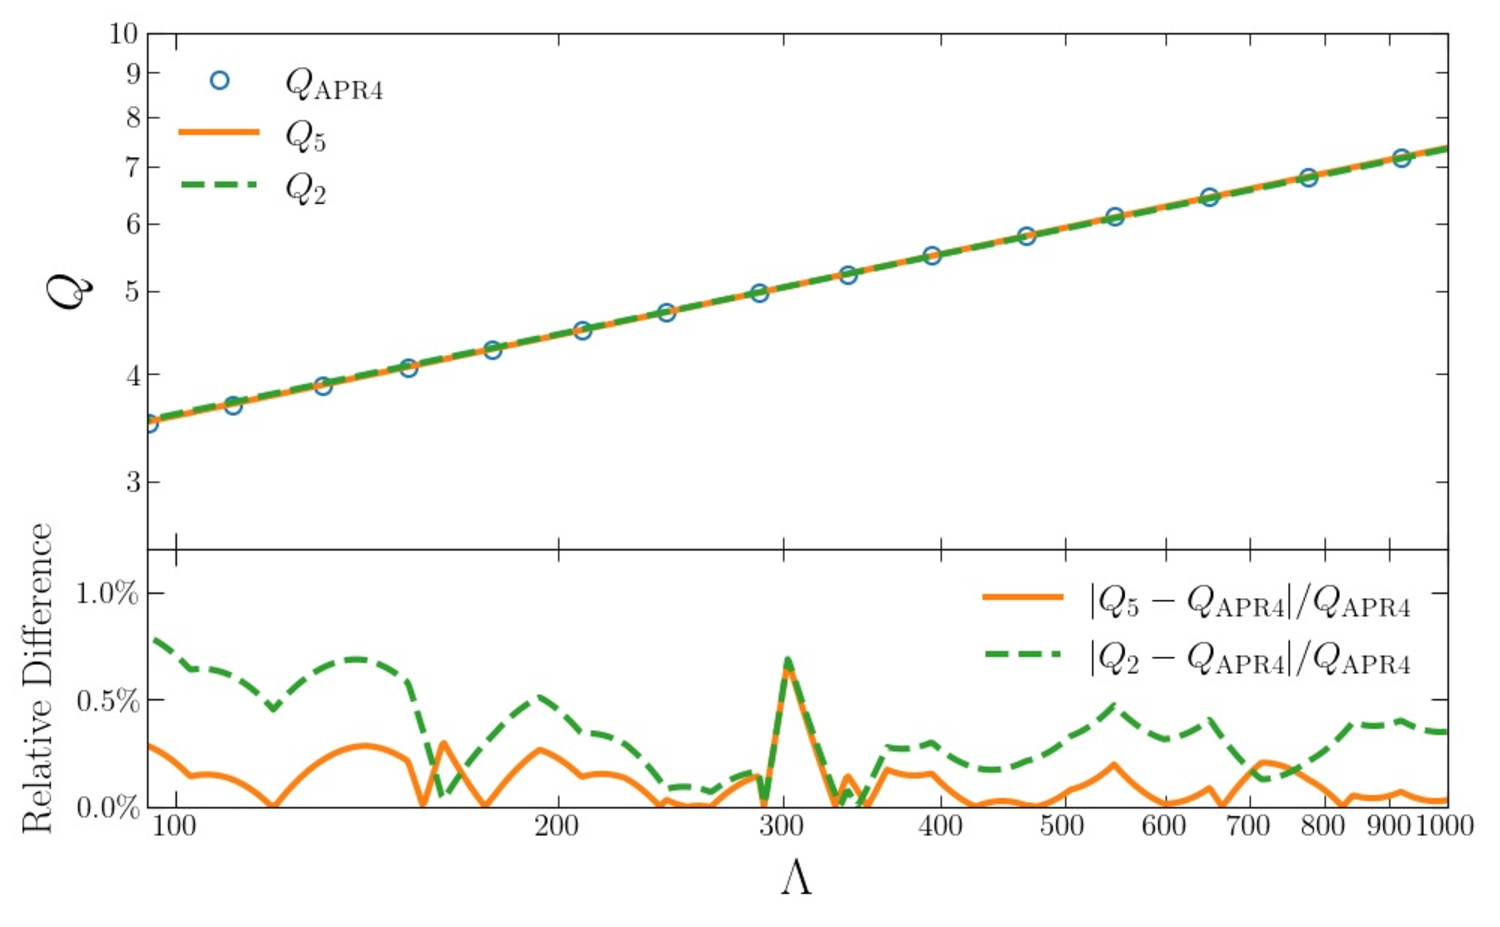
\includegraphics[width=0.8\textwidth]{2d-5d difference.pdf}% Here is how to import EPS art
\caption{\label{relative_difference} The upper panel shows the relation between $\Lambda$ and $Q$ for the Yagi-Yunes relation (Eq.~\eqref{5-d_Love_Q_eq}) and its linear fit (Eq.~\eqref{2-d_Love_Q_eq}). $\Lambda$ and $Q$ calculated assuming APR4 EOS are also plotted as a comparison ($Q_{\mathrm{APR4}}$). The lower panel shows the relative differences.}
\end{figure}

%=============================
\subsection{Principles}
\label{subsec:framework_principles}
%=============================

Hierarchical Bayesian inference is a framework that allows us to combine multiple observations to infer the hyperparameters in a systematic way. In this framework, we want to find the posterior distribution of the hyperparameters $p(\bm{H}|D)$. The data $D=\{d_1,...,d_n\}$ contains data streams $d_i$ of $n$ GW events from the detector network. hyperparameters and single-event parameters are unknown. We apply Bayes' theorem first to obtain the posterior of the hyperparameters $\bm{H}$ and the waveform parameters $\{\bm{\theta}_1,...,\bm{\theta}_n\}$
\begin{equation}
\label{bayes2}
p(\bm{H},\bm{\theta}_1,...,\bm{\theta}_n|D)=\pi(\bm{H},\bm{\theta}_1,...,\bm{\theta}_n)\frac{p(D|\bm{H},\bm{\theta}_1,...,\bm{\theta}_n)}{p(D)}\,,
\end{equation}
where $\pi(\bm{H},\bm{\theta}_1,...,\bm{\theta}_n)$ is the prior probability density for the hyperparameters and waveform parameters, $p(D|\bm{H},\bm{\theta}_1,...,\bm{\theta}_n)$ is the likelihood function, and $p(D)$ is the evidence which we do not need to calculate. To acquire the marginalized posterior for only hyperparameters, we marginalize over the entire parameter space
\begin{equation}
\label{bayes1}
p(\bm{H}|D) = \int p(\bm{H},\bm{\theta}_1,...,\bm{\theta}_n|D) \text{d}\bm{\theta}_1...\text{d}\bm{\theta}_n\,,
\end{equation}

We first consider the priors. Assuming that the $n$ events are independent, the prior can be decomposed into parts of hyperparameters and waveform parameters using the product rule of probability $p(A,B)=p(A)p(B|A)$
\begin{equation}
\label{bayes3}
\pi(\bm{H},\bm{\theta}_1,...,\bm{\theta}_n) = \pi(\bm{H}) \prod_{i=1}^n \pi(\bm{\theta}_i|\bm{H})\,.
\end{equation}

Since Love-Q relation is yet to be determined, we treat tidal deformabilities $\bm{\Lambda}_i=\{\Lambda_{1i},\Lambda_{2i}\}$ and quadrupole moments $\bm{Q}_i=\{Q_{1i},Q_{2i}\}$ as independent variables. Note that Love-Q relation is insensitive to the EOS and we select no particular EOS in the inference part, we assume that the prior distributions for nuisance parameters, including the two mass parameters, are independent of $\bm{\Lambda}_i, \bm{Q}_i$ and $\bm{H}$. 
In this way, the conditional prior for the waveform parameters in Eq.~\eqref{bayes3} can be further decomposed with the product rule
\begin{equation}
\label{prior}
\pi(\bm{\theta}_i|\bm{H})=\pi(\bm{\Lambda}_i|\bm{H})\pi(\bm{Q}_i|\bm{\Lambda}_i,\bm{H})\times\pi(\bm{\xi}_i)\,.
\end{equation}

Analogously to the prior, we decompose the likelihood into a product of single-event likelihoods for $n$ independent BNS observations
\begin{subequations}
\begin{align}
p(D|\bm{H},\bm{\theta}_1,...,\bm{\theta}_n)=\prod_{i=1}^{n}p(\bm{d}_i|\bm{H},\bm{\theta}_i)=\prod_{i=1}^{n}p(\bm{d}_i|\bm{\theta}_i)\,,
\end{align}   
\end{subequations}
note that we have used the fact that the hyperparameters do not enter the waveform thus the likelihood only depends on $\bm{\theta}_i$, i.e., $p(\bm{d}_i|\bm{H},\bm{\theta}_i)=p(\bm{d}_i|\bm{\theta}_i)$.

Based on the derivation above, now the marginalized posterior distribution (Eq.~\eqref{bayes1}) becomes
\begin{equation}
\label{hierarchical bayes}
\begin{aligned}
p(\bm{H}|D)&=\frac{1}{p(D)}\pi(\bm{H})\int \text{d}\bm{\theta}_1...\text{d}\bm{\theta}_n \prod_{i=1}^n \big[\pi(\bm{\Lambda}_i|\bm{H})\pi(\bm{Q}_i|\bm{\Lambda}_i,\bm{H})\pi(\bm{\xi}_i)p(\bm{d}_i|\bm{\theta}_i)\big] \\
&=\frac{1}{p(D)} \pi(\bm{H}) \prod_{i=1}^n
\int \text{d}\bm{\Lambda}_i\text{d}\bm{Q}_i\pi(\bm{\Lambda}_i|\bm{H})\delta\big(\bm{Q}_i-\bm{f}(\bm{\Lambda}_i;\bm{H})\big) \int \text{d}\bm{\xi}_i \pi(\bm{\xi}_i)p(\bm{d}_i|\bm{\theta}_i)\\
&=\frac{1}{p(D)} \pi(\bm{H}) \prod_{i=1}^n
\int \text{d}\bm{\Lambda}_i\pi(\bm{\Lambda}_i|\bm{H})L_i\big(\bm{\Lambda}_i,\bm{f}(\bm{\Lambda}_i;\bm{H})\big)\,,
\end{aligned}
\end{equation}
where the quasi-likelihood function for $\bm{\Lambda}_i,\bm{Q}_i$ is
\begin{equation}
\label{quasi-likelihood}
    L_i(\bm{\Lambda}_i,\bm{Q}_i)=\int \text{d}\bm{\xi}_i \pi(\bm{\xi}_i)p(\bm{d}_i|\bm{\theta}_i)\,.
\end{equation}

%What we need to compute now are the quasi-likelihood functions (eq.~(\ref{quasi-likelihood})) for each GW event and then 
%substitute them into eqs.~(\ref{hierarchical bayes}). Since the hyperparameters $\bm{H}$ do not appear in eq.~(\ref{quasi-likelihood}) 
%and $L_i(\bm{\Lambda}_i,\bm{Q}_i)$ only depend on the data and parameters of the $i\text{-th}$ event, we can perform a single-event Bayesian inference for each event 
%respectively to compute its quasi-likelihood function~\cite{Lackey:2014fwa,Thrane:2018qnx,Golomb:2021tll, Wang:2024xon}. 

In the hierarchical Bayesian framework, the quasi-likelihood of each event can be computed independently on $\bm{H}$. For the $i\text{-th}$ event, we write down Bayes' theorem
\begin{equation}
\label{single bayes}
    p(\bm{\theta}_i|\bm{d}_i)\propto \pi(\bm{\theta}_i|\varnothing)p(\bm{d}_i|\bm{\theta}_i)\,,
\end{equation}
where $\pi(\bm{\theta}_i|\varnothing)$ is regarded as an auxilliary prior independent on $\bm{H}$. $p(\bm{d}_i|\bm{\theta}_i)$ is the single-event likelihood~\cite{Finn:1992wt} given by
\begin{equation}
p(\bm{d}_i|\bm{\theta}_i)\propto \mathrm{e}^{-\frac{1}{2}\langle d_i-h(\bm{\theta}_i),d_i-h(\bm{\theta}_i)\rangle}\,.
\end{equation}
$h(\bm{\theta}_i)$ is given by the waveform model we select. $\langle g, h\rangle$ is the inner product of $g(t)$ and $h(t)$ weighted by the power spectrum density (PSD) of $S_n(f)$ of the noise.
\begin{equation}
    \langle g, h\rangle:= 2\int_{-\infty}^{\infty}\frac{\tilde{g}(f)\tilde{h}^{*}(f)}{S_n(|f|)} \text{d}f\,,
\end{equation}
where $\tilde{g}(f)$ and $\tilde{h}(f)$ are the Fourier transforms of $g(t)$ and $h(t)$.

Rearranging terms of Eq.~\eqref{single bayes} and substituting it into Eq.~\eqref{quasi-likelihood}, we obtain
\begin{equation}
\label{quasi-posterior}
\begin{aligned}
    L_i(\bm{\Lambda}_i,\bm{Q}_i) = \int \text{d}\bm{\xi}_i \pi(\bm{\xi}_i)p(\bm{d}_i|\bm{\theta}_i) \propto \int \text{d}\bm{\xi}_i \frac{\pi(\bm{\xi}_i)}{\pi(\bm{\theta}_i|\varnothing)}p(\bm{\theta}_i|\bm{d}_i)\,.
\end{aligned}  
\end{equation}
If we choose single-event prior $\pi(\bm{\theta}_i|\varnothing)\propto\pi(\bm{\xi}_i)$, i.e., a flat prior for $\bm{\Lambda}_i$ and $\bm{Q}_i$, Eq.~\eqref{quasi-posterior} can be further simplified as 
\begin{equation}
\label{quasi-marginalized}
\begin{aligned}
    L_i(\bm{\Lambda}_i,\bm{Q}_i) \propto \int \text{d}\bm{\xi}_i p(\bm{\theta}_i|\bm{d}_i)\propto p(\bm{\Lambda}_i,\bm{Q}_i|\bm{d}_i)\,.
\end{aligned}  
\end{equation}
We find that under this choice of prior, the quasi-likelihood is proportional to the marginalized posterior for the single-event inference. Now we can see that the hierarchical Bayesian framework, as its name implies, introduces two levels of inference for the single-event parameters and the hyperparameters. The first level consists of single-event Bayesian inferences, based on Eq.~\eqref{single bayes}. The second is the hyperparameter inference, based on Eq.~\eqref{hierarchical bayes}. As a bridge connecting these two levels of inference, Eq.~\eqref{quasi-marginalized} allows us to construct the quasi-likelihoods with the marginalized posteriors obtained from single-event inferences.


%=============================
\section{Simulation}
\label{sec:simulation}
%=============================

%=============================
\subsection{Waveform, Population and Detectors}
\label{subsec:simulation_preliminaries}
%=============================

For our simulation, we adopt the {\sc imrphenomxas\_nrtidalv3} waveform model~\cite{Abac:2023ujg}, which is an aligned spin waveform model and includes tidal amplitude corrections as well as spin-induced quadrupole moment terms up to 3.5PN. The parameter set is composed of the binary masses $m_1$ and $m_2$, the dimensionless tidal deformabilities $\Lambda_1$ and $\Lambda_2$ and spin-induced quadrupole moments $Q_1$ and $Q_2$ of each component, the dimensionless spin aligned with the direction of the orbital angular momentum $\chi_i$, the luminosity distance $D_L$, the merge time $t_c$, the right ascension $\alpha$ and declination $\delta$, the inclination angle $\iota$, the GW polarization angle $\psi$ and the phase of coalescence $\phi_c$. We denote the entire parameter set as a vector $\bm{\theta}$, i.e.,
\begin{equation}
\label{parameter set}
\bm{\theta} = \{m_1,m_2,\Lambda_1,\Lambda_2,Q_1,Q_2,\chi_1,\chi_2,D_L,t_c,\alpha,\delta,\iota,\psi,\phi_c\}\,.
\end{equation}

We adopt the BNS mass population model proposed by Farrow~et~al.~\cite{Farrow:2019xnc}. According to their spin magnitude, the model divides BNS into a recycled star and a nonrecycled (\emph{slow}) one, for which the masses are labeled $m_r$ and $m_s$, respectively. The distribution of $m_r$ has two Gaussian components while $m_s$ follow a uniform distribution,
\begin{subequations}
\label{mass population}
\begin{equation}
    P(m_r) = \alpha \mathcal{N}(\mu_1, \sigma_1) + (1-\alpha) \mathcal{N}(\mu_2, \sigma_2)\,,
\end{equation}
\begin{equation}
    P(m_s) = \mathcal{U}(m_s^l, m_s^u)\,,
\end{equation}
\end{subequations}
where $\alpha=0.68$, $\mu_1=1.34\mathrm{M}_{\odot}$, $\sigma_1=0.02\mathrm{M}_{\odot}$, $\mu_2=1.47\mathrm{M}_{\odot}$, $\sigma_2=0.15\mathrm{M}_{\odot}$ and $m_s^l=1.14\mathrm{M}_{\odot}$, $m_s^u=1.46\mathrm{M}_{\odot}$. When generating simulation GW signals, for each event we just select the larger one of $m_r$ and $m_s$ as the primary mass $m_1$ and the other as the secondary mass $m_2$, since we always demand $m_1 \geq m_2$.

The tidal deformability and quadrupole moments of the binary are calculated from the stellar mass assuming the APR4 EOS. Refs.~\cite{Yagi:2013awa,Atta:2024ckt} demonstrates in detail how to derive tidal deformability $\Lambda_i$ and quadrupole moment $Q_i$ given the mass $m_i$ and the EOS. For the dimensionless spin component $\chi_r$ of recycled stars, we adopt a uniform distribution $\mathcal{U}(-0.5,0.5)$, 
while in the case of slow stars, the spin $\chi_s$ is drawn from $\mathcal{U}(-0.1,0.1)$.

Using the cosmological parameters provided by the Planck Collaboration~\cite{Planck:2018vyg}, we simulate 1000 GW sources distributed uniformly in co-moving volume from 15Mpc to 150Mpc~\cite{Fishbach:2018edt,KAGRA:2021duu}, with isotropic sky locations and orientations. This corresponds to the observed local merger rate $7.6$--$250\,\mathrm{Gpc}^{-3}\mathrm{yr}^{-1}$ from current GW detections~\cite{LIGOScientific:2025pvj,LIGOScientific:2020aai}. Without loss of generality, all these GW events are injected with an arbitrary coalescence time $t_c=0$.

We select a ground based network consisting of two CE detectors and one ET detector. We use the noise curves of the CE and ET detectors with the CE-2~\cite{Reitze:2019iox,Reitze:2019dyk} and ET-D~\cite{Punturo:2010zz,Hild:2010id,Sathyaprakash:2012jk} configurations respectively. The two CE detectors are positioned at the current sites of the two LIGO detectors, while the ET detector is set at the current location of the Virgo detector with a triangular shape. 

%=============================
\subsection{Implementation}
\label{subsec:simulation_implementation}
%=============================

The evaluation of the marginalized posterior for hyperparameters can be divided into two steps, according to the discussion in section~\ref{subsec:framework_principles}. We firstly perform Bayesian inference for each event. The quasi-likelihood (Eq.~\eqref{quasi-posterior}) can be obtain through a density estimation method introduced by Ref.~\cite{Talbot:2020oeu}; 
then we substitute the quasi-likelihoods into Eq.~\eqref{hierarchical bayes} and finish the integral as the likelihood of the hyperparameter inference. Secondly, we conduct another sampling procedure to finally obtain the posterior samples of hyperparameters with flat priors. 

In the first step, when conducting single-event Bayesian inference, we choose $\mathcal{M}$ and $\eta$ as mass parameters. In this way, the parameter set of single-event Bayesian inference becomes $\bm{\theta} = \{\mathcal{M},\eta,\Lambda_1,\Lambda_2,Q_1,Q_2,\chi_1,\chi_2,D_L,t_c,\alpha,\delta,\iota,\psi,\phi_c\}$. The priors of $\mathcal{M},\eta,\chi_1,\chi_2,t_c,\phi_c$ are uniform, while the prior of $D_L$ is uniform in the co-moving volume and source frame time. We set isotropic priors for the angle variables $\alpha,\delta,\iota,\psi$. For tidal and quadrupole moment parameters, we treat $\Lambda_s$ and $Q_s$ of the slow binary component as nuisance parameters, considering that the spin-induced quadrupole moment is poorly estimated with low spin~\cite{Yagi:2013awa}. We select uniform priors for $\Lambda_1,\Lambda_2$ and $Q_1,Q_2$ and now Eq.~\eqref{quasi-posterior} becomes
\begin{equation}
    \label{quasi-marginalized1}
    \begin{aligned}
        L_i(\Lambda_{ri},Q_{ri}) \propto p(\Lambda_{ri},Q_{ri}|\bm{d}_i)\,,
    \end{aligned}  
\end{equation}
where $\Lambda_{ri}$ and $Q_{ri}$ are the tidal deformability and quadrupole moment of the recycled binary component of the $i$-th event, respectively. Eq.~\eqref{quasi-marginalized} reveals that the quasi-likelihood is proportional to the marginalized posterior $p(\Lambda_{ri},Q_{ri}|\bm{d}_i)$, indicating that we can directly construct the quasi-likelihood from posterior samples.

After sampling, we obtain the quasi-likelihood of each event from $\Lambda_r$ and $Q_r$ samples. To complete the integral in Eq.~\eqref{hierarchical bayes}, we must create a functional form for each quasi-likelihood using the posterior samples. Following Golomb and Talbot~\cite{Golomb:2021tll}, we adopt the Gaussian mixture model (GMM) method developed by Ref.~\cite{Talbot:2020oeu} as the density estimation method to obtain the quasi-likelihood with Eq.~\eqref{quasi-likelihood}. Substitute the results of density estimation into Eq.~\eqref{hierarchical bayes}, and then the likelihood function of the hyperparameter estimation can be constructed.

In the second step, we sample the integrand of Eq.~\eqref{hierarchical bayes} with Bayesian inference. For hyperparameters $\pi(\bm{H})$, we use uniform priors with the boundaries listed in table~\ref{prior_table} and for the prior $\pi(\bm{\Lambda}_i|\bm{H})$, we use the uniform distribution $\mathcal{U}(10,2000)$. For Bayesian inference in both steps, posterior samples are generated with {\sc NESSAI}~\cite{Skilling:2004pqw,Skilling:2006gxv,michael_j_williams_2025_14627250,PhysRevD.103.103006,Williams:2023ppp} of the {\sc BILBY}~\cite{Ashton:2018jfp} package. We simulate 1000 GW events as described in section~\ref{subsec:simulation_preliminaries}. 

Ref.~\cite{Lackey:2014fwa} found that the overwhelming majority of the information for population properties comes from the events with the highest SNRs and Ref.~\cite{Yagi:2013awa} concluded that the spin-induced quadrupole moment is poorly estimated with a low spin. Considering these findings, we only pick some of the simulated GW sources and leave the full-population study for future work. In practice, we first draw 100 sources with the highest SNRs; then among these 100 sources we further select 20 sources whose recycled components rotate the fastest (i.e., with the largest $|\chi_{ri}|$). 

\begin{table}[htbp]
    \centering
    \sisetup{
        table-align-text-post = false, 
        separate-uncertainty = true 
    }
    \caption{\label{prior_table}The best fit values of Yagi-Yunes relation and the priors of the hyperparameters in different polynomial models with $j=2, 3, 4, 5$ parameters for the Bayesian inference. The best fit values are calculated as direct fittings of the Yagi-Yunes relation with different polynomial models and are regarded as reference values in our inference.}
    \begin{tabular}{
        l
        S[table-format=-1.4]
        S[table-format=1.5]
        S[table-format=1.3e-1]
        S[table-format=-1.3e-1]
        S[table-format=1.3e-1]
    }
        \toprule
        \multicolumn{6}{c}{Best fit values} \\
        %\cmidrule(l){2-6}
        $j$ & {$a_j$} & {$b_j$} & {$c_j$} & {$d_j$} & {$e_j$} \\
        \midrule

        5 \, &  0.1940 & 0.0916 & 4.812e-2 & -4.283e-3 & 1.245e-4 \\
        4 \, &  0.1290 & 0.1480  & 3.021e-2 & -1.817e-3 & {/}      \\
        3 \, & -0.0709 & 0.2775  & 3.220e-3 & {/}       & {/}      \\
        2 \, & -0.1457 & 0.3094  & {/}      & {/}       & {/}      \\
        
        \midrule

        \multicolumn{6}{c}{Priors} \\
        %\cmidrule(l){2-6}
        $j$ & {$a_j$} & {$b_j$} & {$c_j$} & {$d_j$} & {$e_j$} \\
        \midrule

        5 \, & {$\mathcal{U}(-5.0, 5.0)$} & {$\mathcal{U}(-1.0, 1.0)$} & {$\mathcal{U}(-0.5, 0.5)$} & {$\mathcal{U}(-0.1, 0.1)$} & {$\mathcal{U}(-0.01, 0.01)$} \\
        4 \, & {$\mathcal{U}(-5.0, 5.0)$} & {$\mathcal{U}(-1.0, 1.0)$} & {$\mathcal{U}(-0.5, 0.5)$} & {$\mathcal{U}(-0.1, 0.1)$} & {/}                         \\
        3 \, & {$\mathcal{U}(-5.0, 5.0)$} & {$\mathcal{U}(-1.0, 1.0)$} & {$\mathcal{U}(-0.5, 0.5)$} & {/}                       & {/}                         \\
        2 \, & {$\mathcal{U}(-5.0, 5.0)$} & {$\mathcal{U}(-1.0, 1.0)$} & {/}                       & {/}                       & {/}                         \\
        \bottomrule
    \end{tabular}
\end{table}


%=============================
\section{Results and Discussions}
\label{sec:results}
%=============================
%\ZW{I'm not recommend to use ``sec4'' to label the section, because it is not informative. Also for equation labels, since the index may change when you revise the paper, it is better to use some informative labels, e.g., ``sec:results and discussions''}
In this section, we present the inference results for different parameterization models of the Love-Q relation. In section~\ref{subsec:results_linear_model}, we show the results of the linear model, Eq.~\eqref{2-d_Love_Q_eq}, consisting of two parameters.
%\ZW{Another question: All eq. should be replaced by Eq. There is no additional ``.'' after figure and table, e.g., figure~\ref{corner2-d}, table~\ref{prior_table}.} 
In section~\ref{subsec:results_quartic}, we present the results of the quartic polynomial model in Eq.~\eqref{5-d_Love_Q_eq}, consisting of five parameters. The polynomial models in between, i.e., the quadratic and cubic polynomial models, are discussed in section~\ref{subsec:results_quadratic_cubic}.
%=============================
\subsection{Linear Model}
\label{subsec:results_linear_model}
%=============================
%\ZW{I delete ``fitting'', since it is not informative.}
\begin{figure}
    \centering
    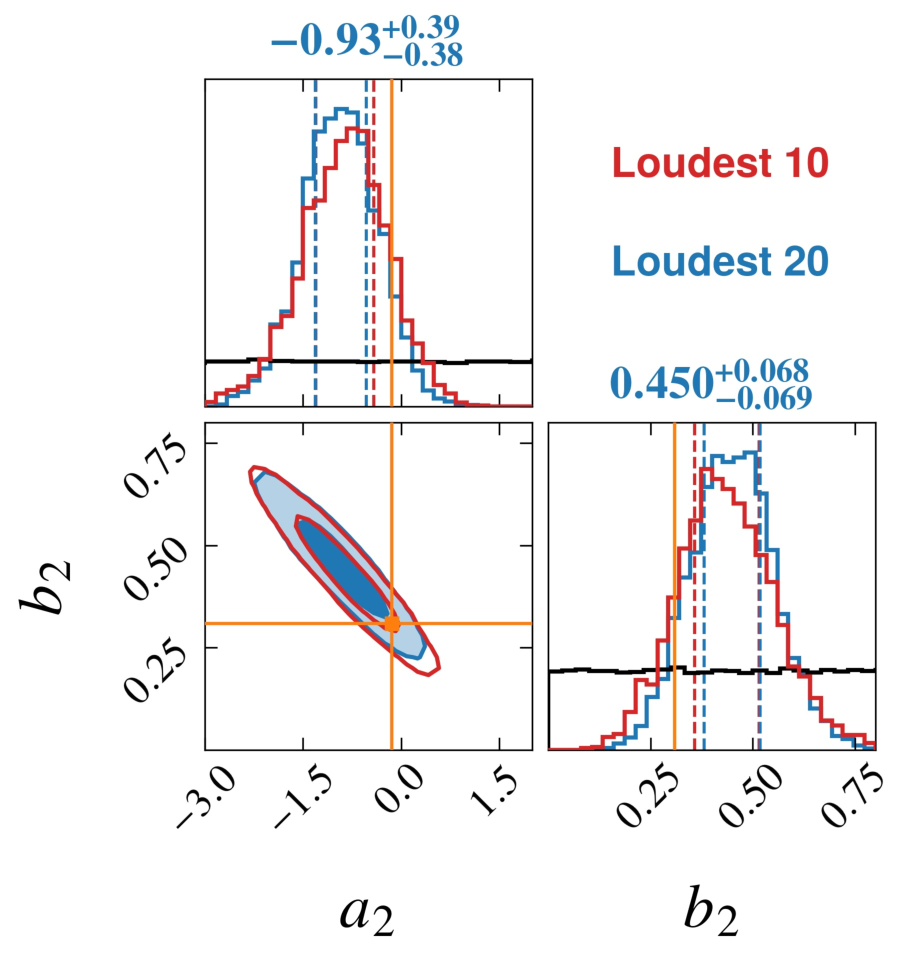
\includegraphics[width=0.5\linewidth]{comparison_corner_plot.pdf}
    \caption{Posterior distributions of the hyperparameters in the linear fitting case. The contours refer to 50\% and 90\% credible regions for both inferences based on the loudest 10 and 20 events. The numbers above the histograms stand for the median and the central 50\% credible interval of each marginalized distribution in the 20 event inference. The orange lines represent the best fit values of the parameters in table~\ref{prior_table}. The priors are also drawn in black for the histograms on the diagonal.}
    \label{corner2-d}
\end{figure}

\begin{figure}
\centering
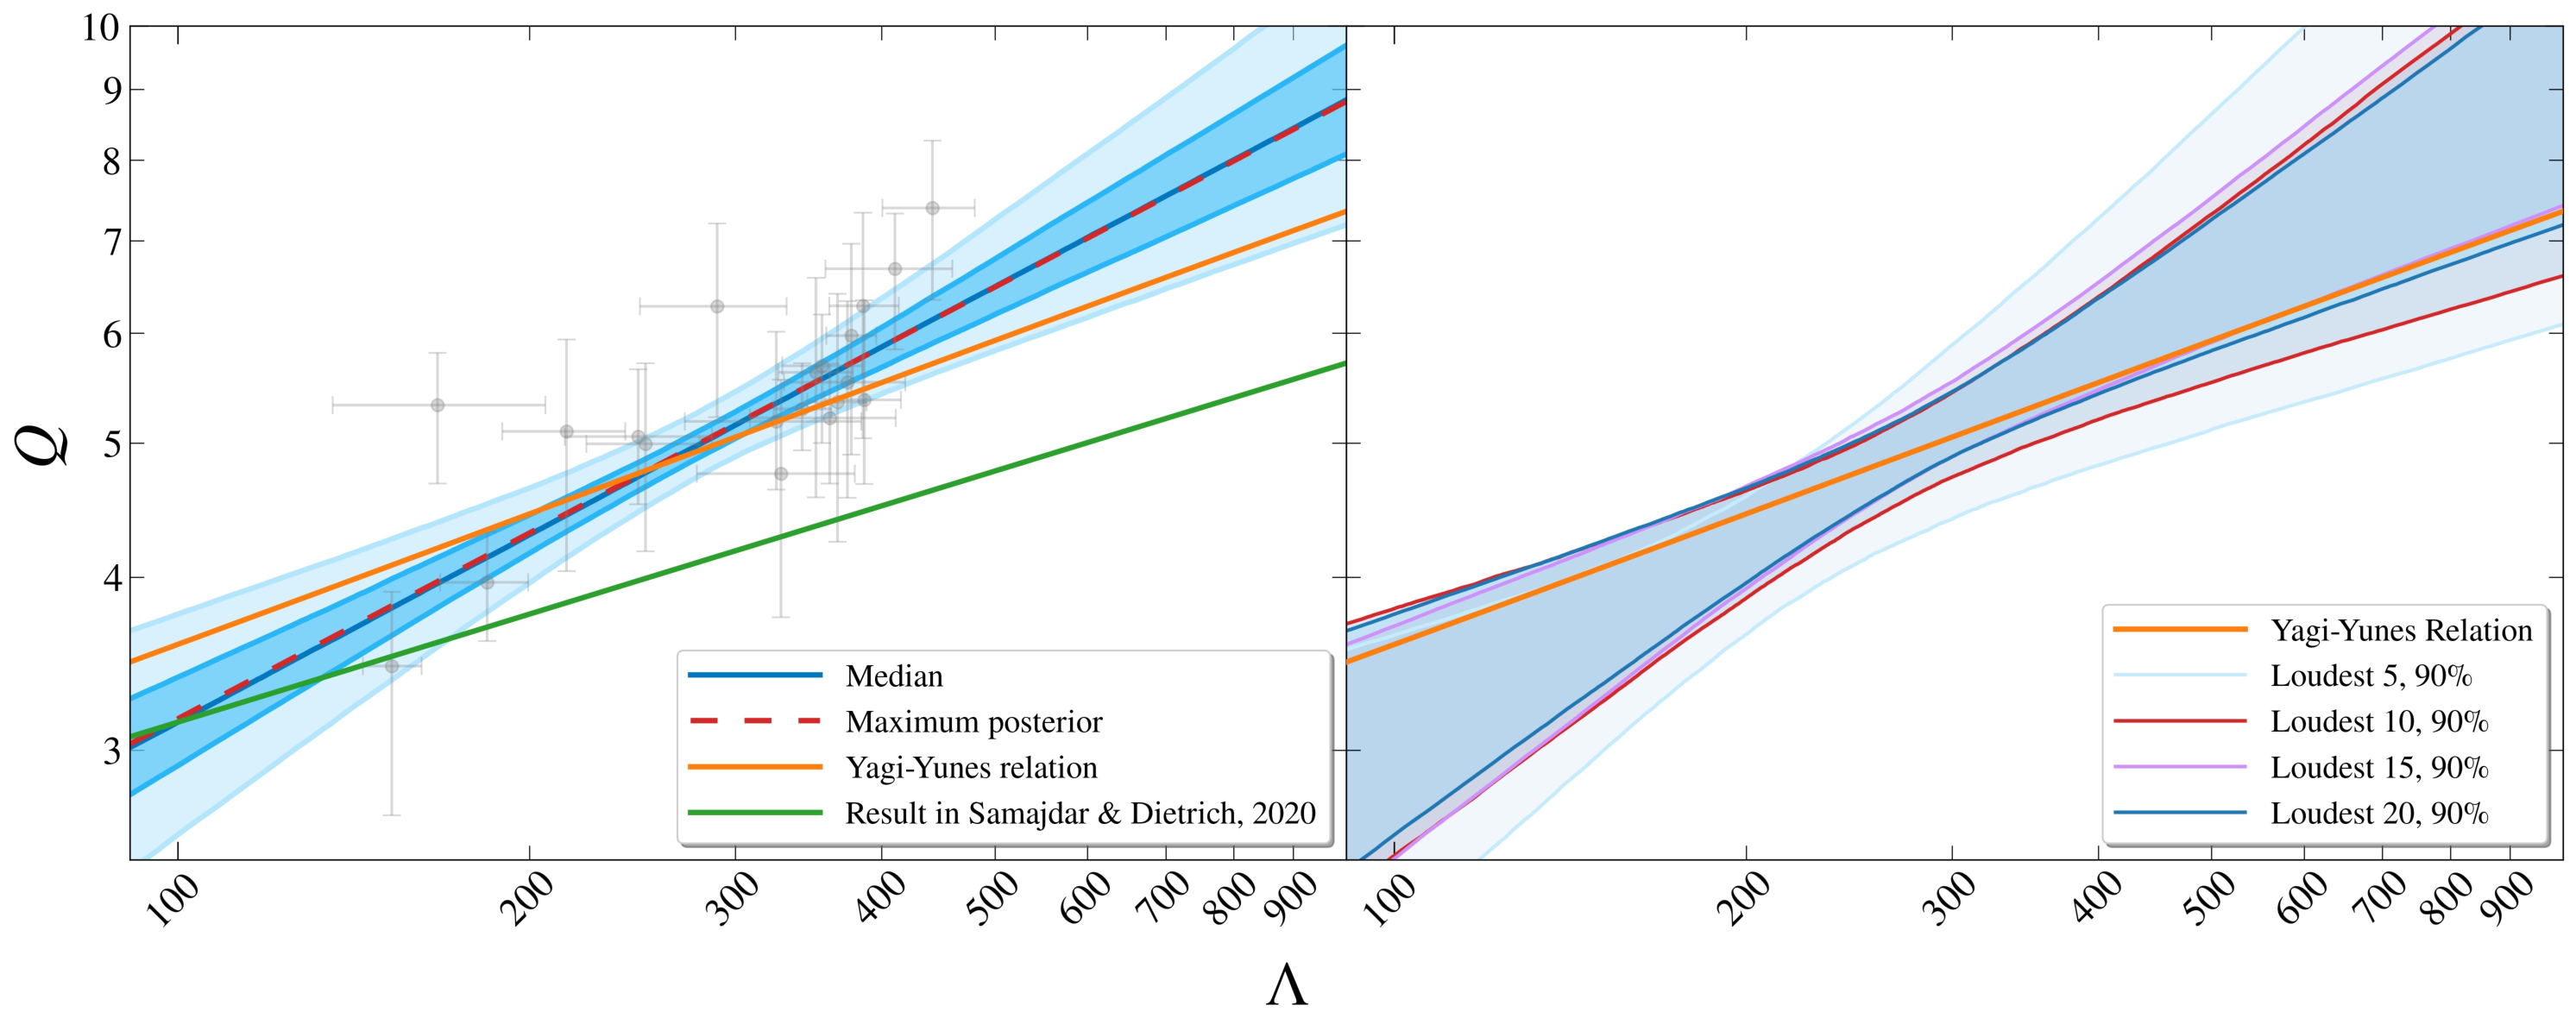
\includegraphics[width=\textwidth]{hierarchical_results_APR4_2d.pdf}
    \caption{Results of the hierarchical Bayesian inference for linear Love-Q relation. In the left panel, the Love-Q relation is inferred based on 20 simulated GW events. The gray error bars demonstrate the $1\sigma$ credible interval of $\Lambda$ and $Q$. The orange solid line represents the Yagi-Yunes Love-Q relation and the green solid line refs to the result given by Samajdar \& Dietrich, 2020~\cite{Samajdar:2020xrd}. The blue regions from dark to light represent the $50\%$ and $90\%$ credible intervals of $Q$. The blue solid line and the red dashed line are the median and peak of the distribution of $Q$ with certain $\Lambda$. In the right panel, contours correspond to $90\%$ credible intervals for the inference result based on the loudest 5, 10, 15, 20 events, respectively.
    \label{2-d_Love_Q}}
\end{figure}
We first perform the inference for the linear model, which is also the model adopted in Ref.~\cite{Samajdar:2020xrd}. The posterior distribution of the hyperparameters $\{a_2,b_2\}$ is shown in figure~\ref{corner2-d}. Compared
to the priors in table~\ref{prior_table}, the posteriors are significantly narrowed. As a comparison, we also mark the fitting values of the hyperparameters in a direct fit of the Yagi-Yunes Love-Q relation, and regard them as ``true'' values of the linear model for reference. These values fall within the 90\% credible region of the posterior, and close to the marginal of the 50\% credible region. The hierarchical Bayesian inference successfully recovers the Love-Q relation under the linear parameterization. We also investigate how the results depend on the number of events in the analysis. In the 20 event selected in section~\ref{subsec:simulation_implementation}, we further select the loudest 10 events, perform the inference again, and show the results in figure~\ref{corner2-d}. For both the joint and marginalized distributions, the widths of the credible regions in the 10-event inference are only slightly larger than those in the 20-event inference. This reveals that the loudest 10 events dominate the information in constraining the Love-Q relation, and including quieter events will not significantly improve the results.

In figure~\ref{2-d_Love_Q}, we show the recovered Love-Q relation according to the posterior samples. For each $\Lambda$, every sample in the posterior of the hyperparameters corresponds to a $Q$ value. With $\Lambda$ fixed, we find the credible intervals of $Q$, and then vary $\Lambda$ continuously to form credible regions. In the left panel, we show the results of the 20-event inference. Similar to figure~\ref{corner2-d}, the Yagi-Yunes Love-Q relation is
covered by the 90\% credible region. In the right panel, we select the loudest 5, 10, 15 and 20 events from the 20 events to test how the recovered Love-Q relation depends on the number of events. We find the widths of the 90\% credible regions are almost the same for the 10, 15 and 20 event inferences. This is consistent with the posteriors in figure~\ref{corner2-d}, and again indicates that the loudest 10 events are almost sufficient to constrain the Love-Q relation. Similar phenomena were also found in previous studies~\cite{Lackey:2014fwa,Wang:2024xon}, where the recovered $\Lambda$-$m$ relation were also dominated by the several loudest events.

%=============================
\subsection{Quartic Polynomial Model}
\label{subsec:results_quartic}
%=============================

\begin{figure}
\begin{minipage}[t]{0.49\textwidth}
\centering
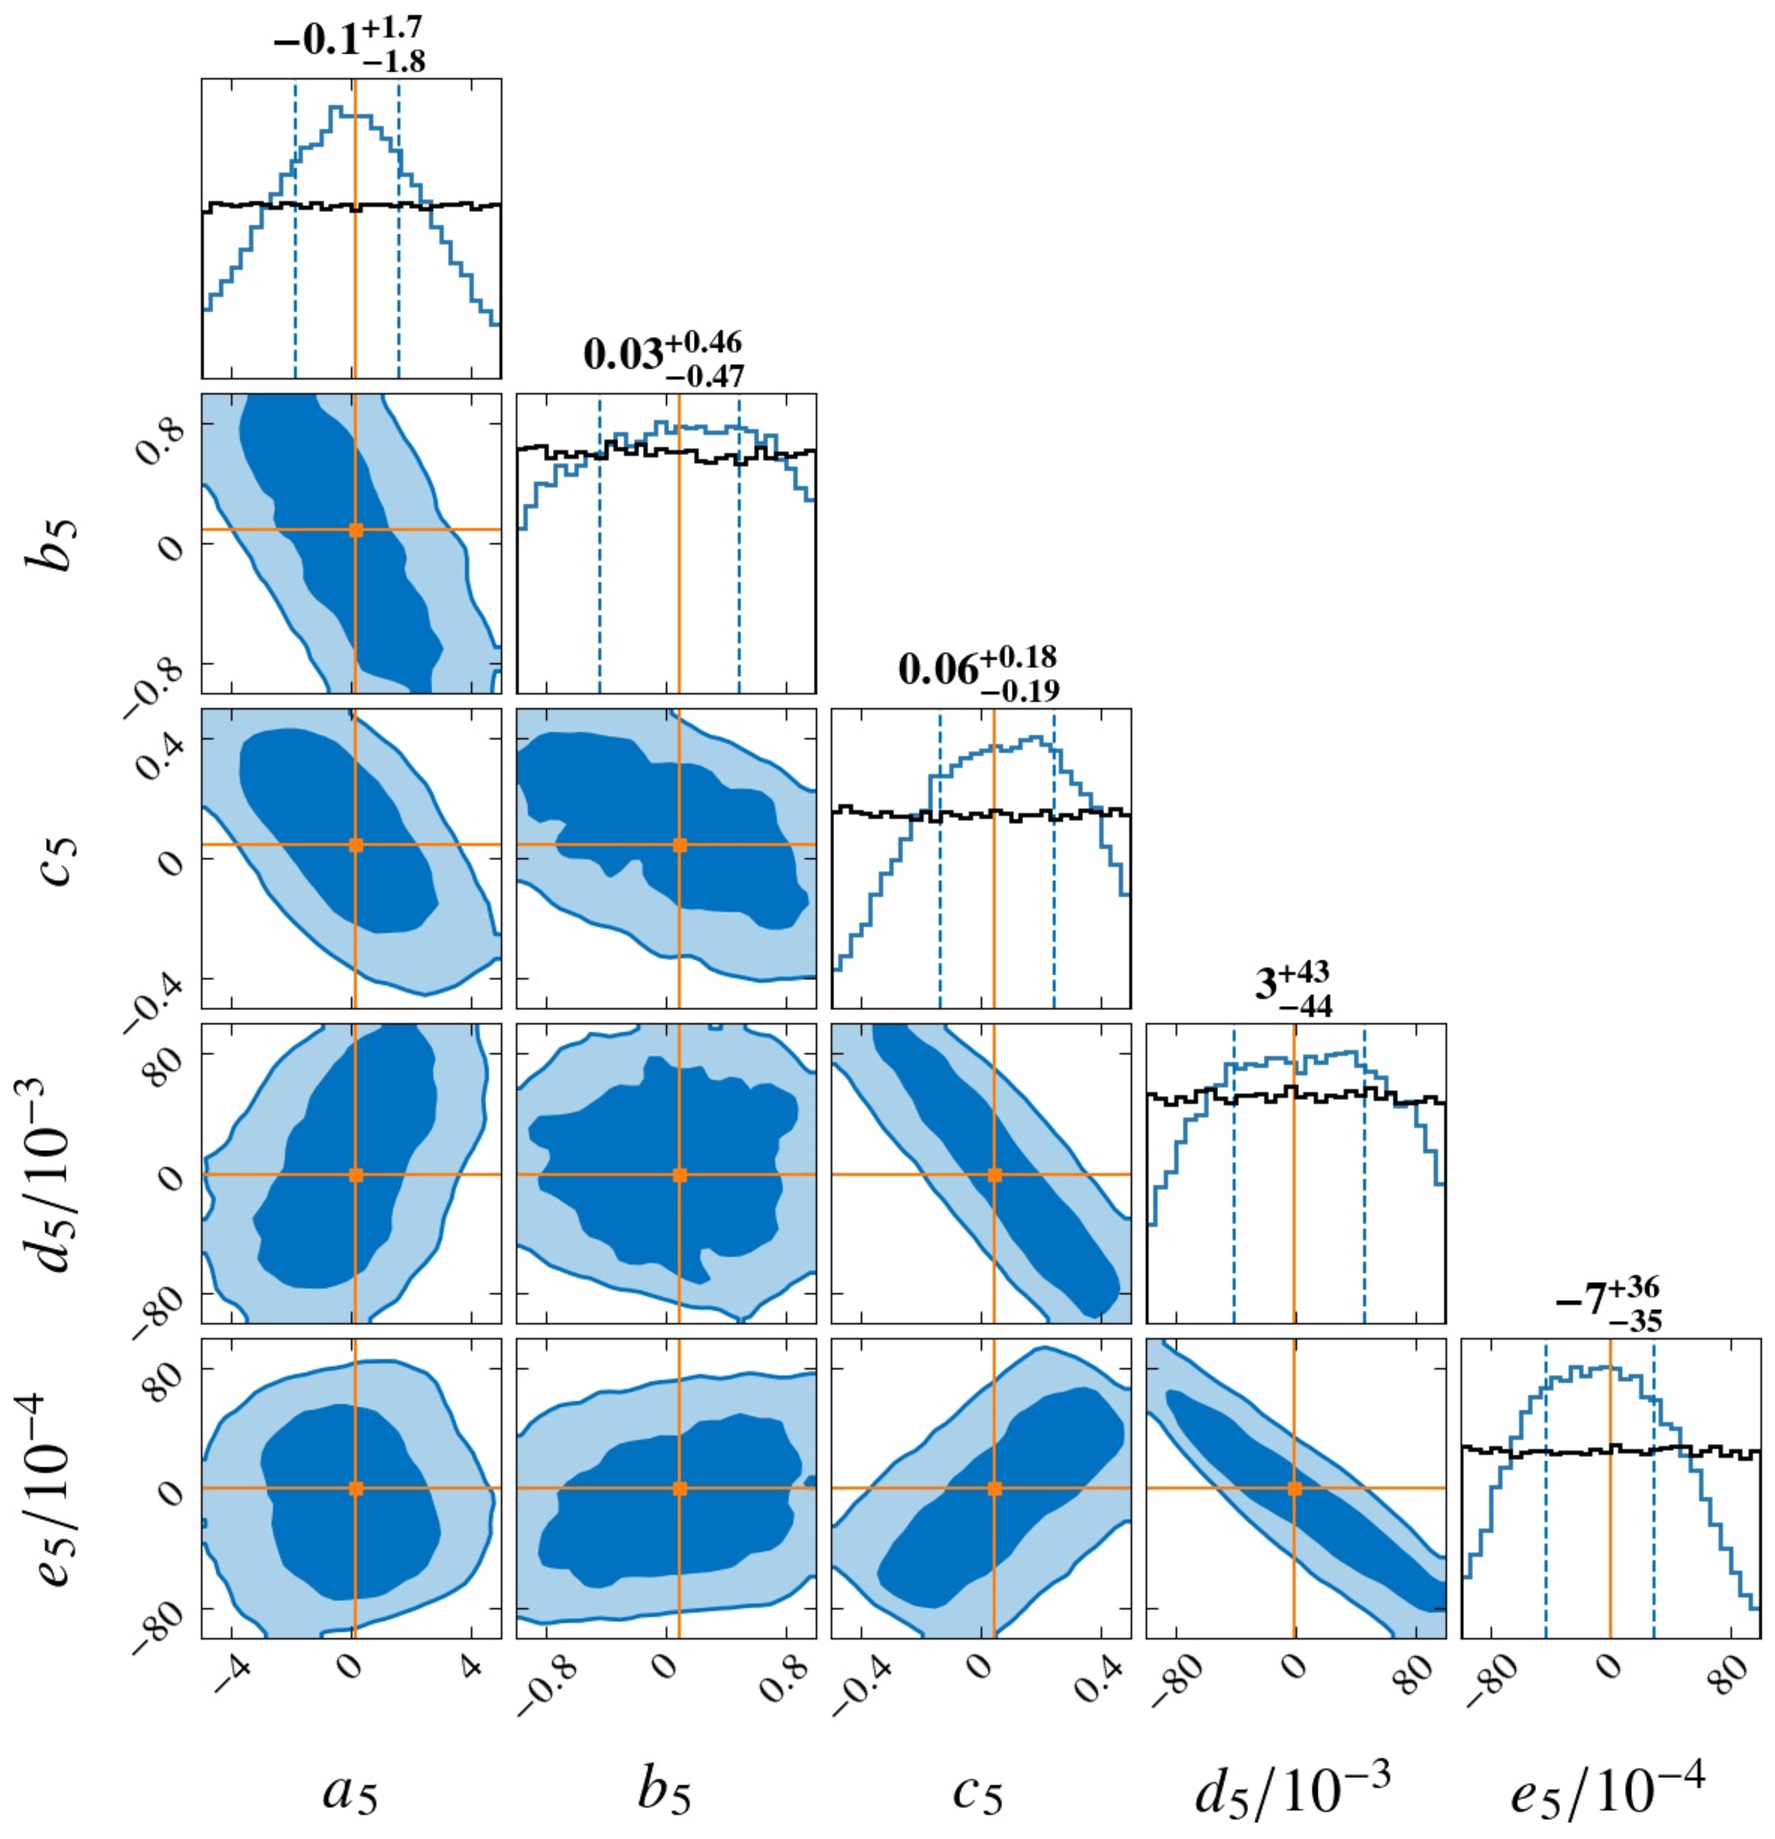
\includegraphics[width=0.8\linewidth]{Hyper_parameter_5d.pdf}% Here is how to import EPS art
\end{minipage}
\hfill
\begin{minipage}[t]{0.49\textwidth}
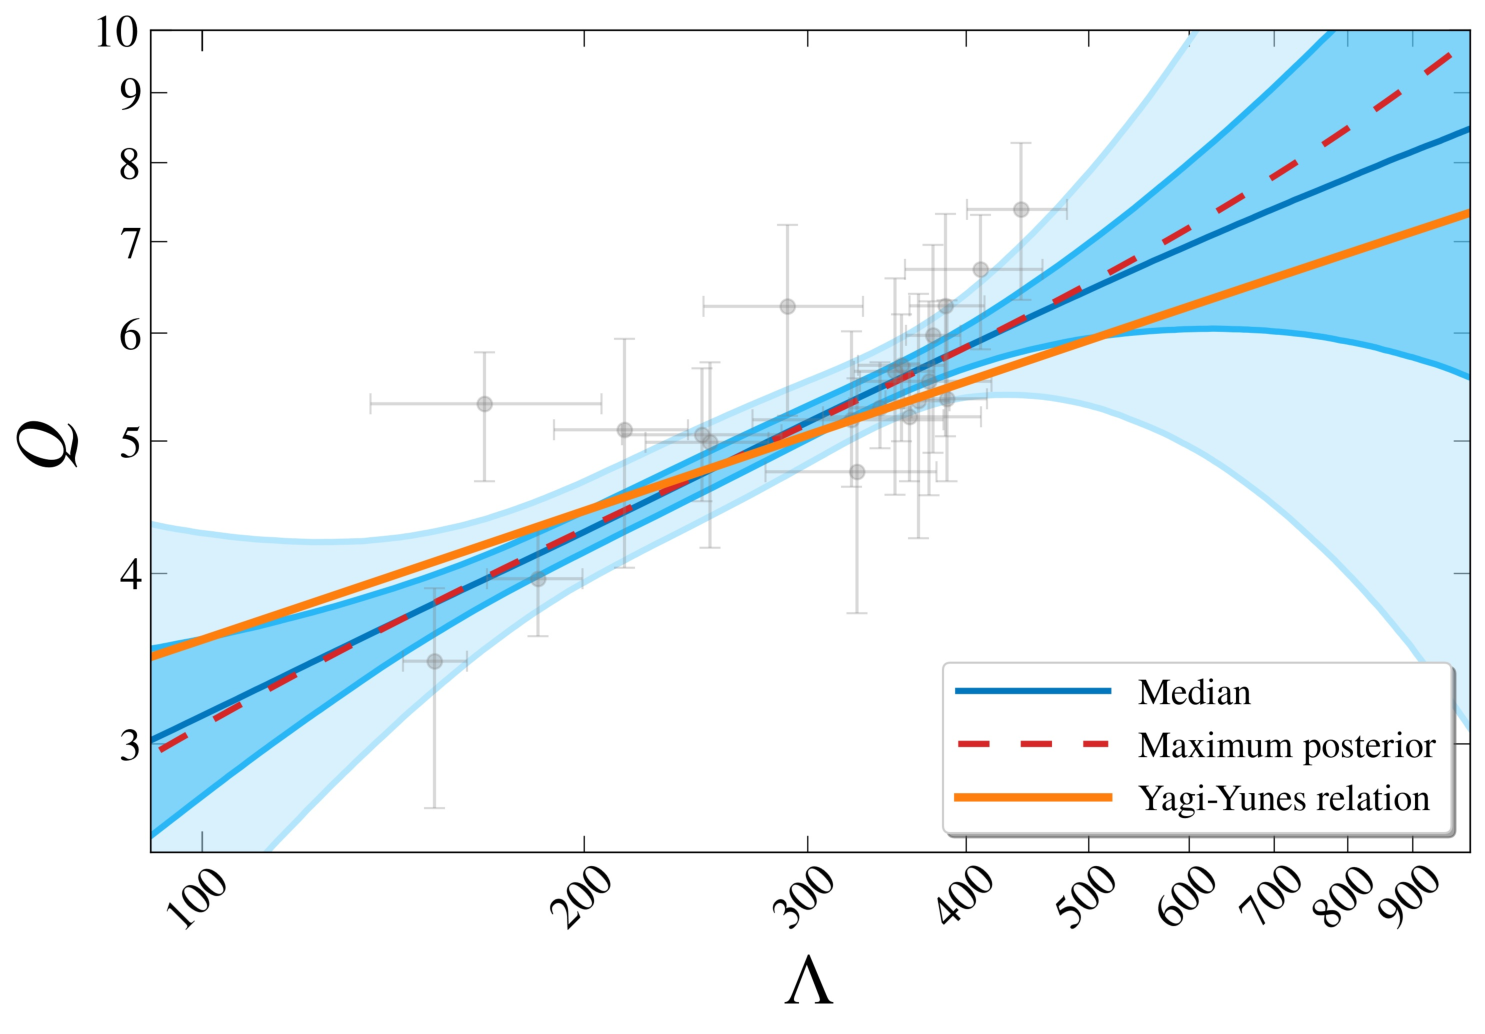
\includegraphics[width=\linewidth]{hierarchical_results_APR4_5d.pdf}
\end{minipage}
    \caption{\label{5-d_Love_Q} Left panel: posterior distribution of the hyperparameters in the quartic polynomial model. The inference is based on all of the 20 events. The orange lines represent the values in the Yagi-Yunes Love-Q relation. Right panel: similar to figure~\ref{2-d_Love_Q}, but for the quartic polynomial model. Still, the Yagi-Yunes Love-Q relation is included in the $90\%$ credible region.} 
\end{figure}

For the quartic polynomial model, the Love-Q relation is fitted with five parameters shown in Eq.~\eqref{5-d_Love_Q_eq}, i.e., $\{a_5, b_5, c_5, d_5, e_5\}$. This is also the original model proposed by Yagi and Yunes~\cite{Yagi:2013awa}. We summarize the posterior and the recovered Love-Q relation in figure~\ref{5-d_Love_Q}, where
all 20 events are included in the inference. In the left panel, though the true values (the values in Yagi-Yunes Love-Q
relation~\cite{Yagi:2013awa}) are almost centered in the 50\% and 90\% credible regions, the posteriors are much wider than those in the linear case, reaching the prior boundaries. This indicates that the $\Lambda$ and $Q$ measurements
from these events are not informative enough to well constrain all the five parameters. In other words, the observation precision is not high enough to capture the higher-order terms introduced by the additional three parameters
$c_5, d_5$ and $e_5$. This is also reflected in the strong correlations between the three parameter shown in the left panel of figure~\ref{5-d_Love_Q}. In the right panel of figure~\ref{5-d_Love_Q}, the 90\% credible regions of the
recovered Love-Q relation are also wider than those in the linear case, especially for large $\Lambda$ where the higher-order terms become more important. For $\Lambda \sim 400$, the widths of the 90\% credible region between
the two models are similar, which is consistent with the fact that most of the simulated events gather around this region. The Yagi-Yunes Love-Q relation is mostly covered by the 50\% credible region, and well within the 90\% credible region.

%=============================
\subsection{Quadratic and Cubic Polynomial Models}
\label{subsec:results_quadratic_cubic}
%=============================

\begin{figure}
    \begin{minipage}[t]{0.49\textwidth}
    \centering
    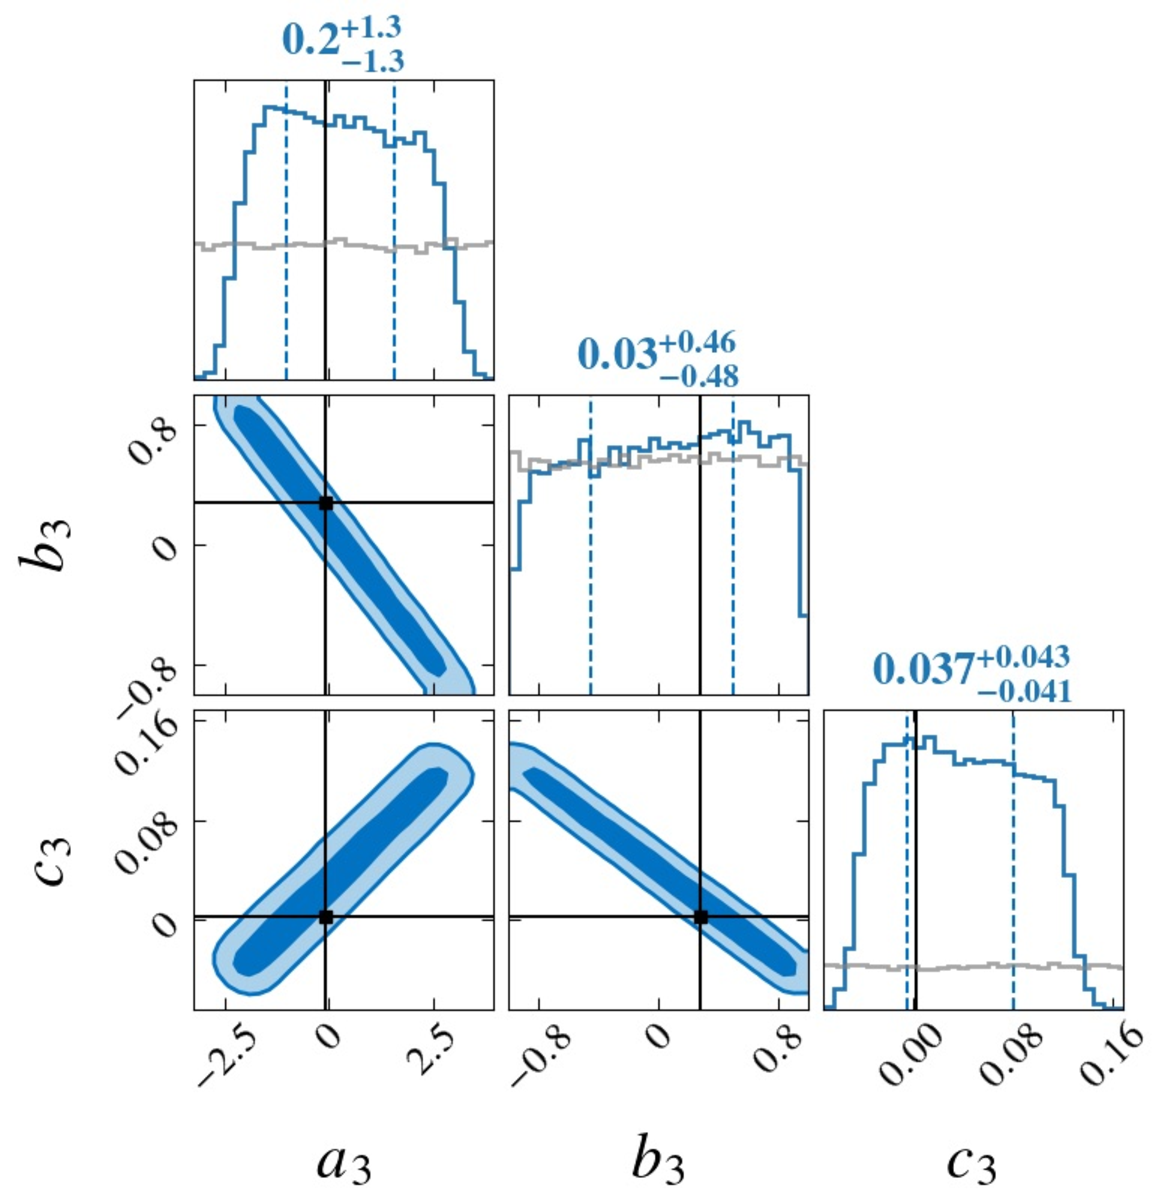
\includegraphics[width=0.8\linewidth]{Hyper_parameter_3d.pdf}
    \end{minipage}
    \hfill
    \begin{minipage}[t]{0.49\textwidth}
    \centering
    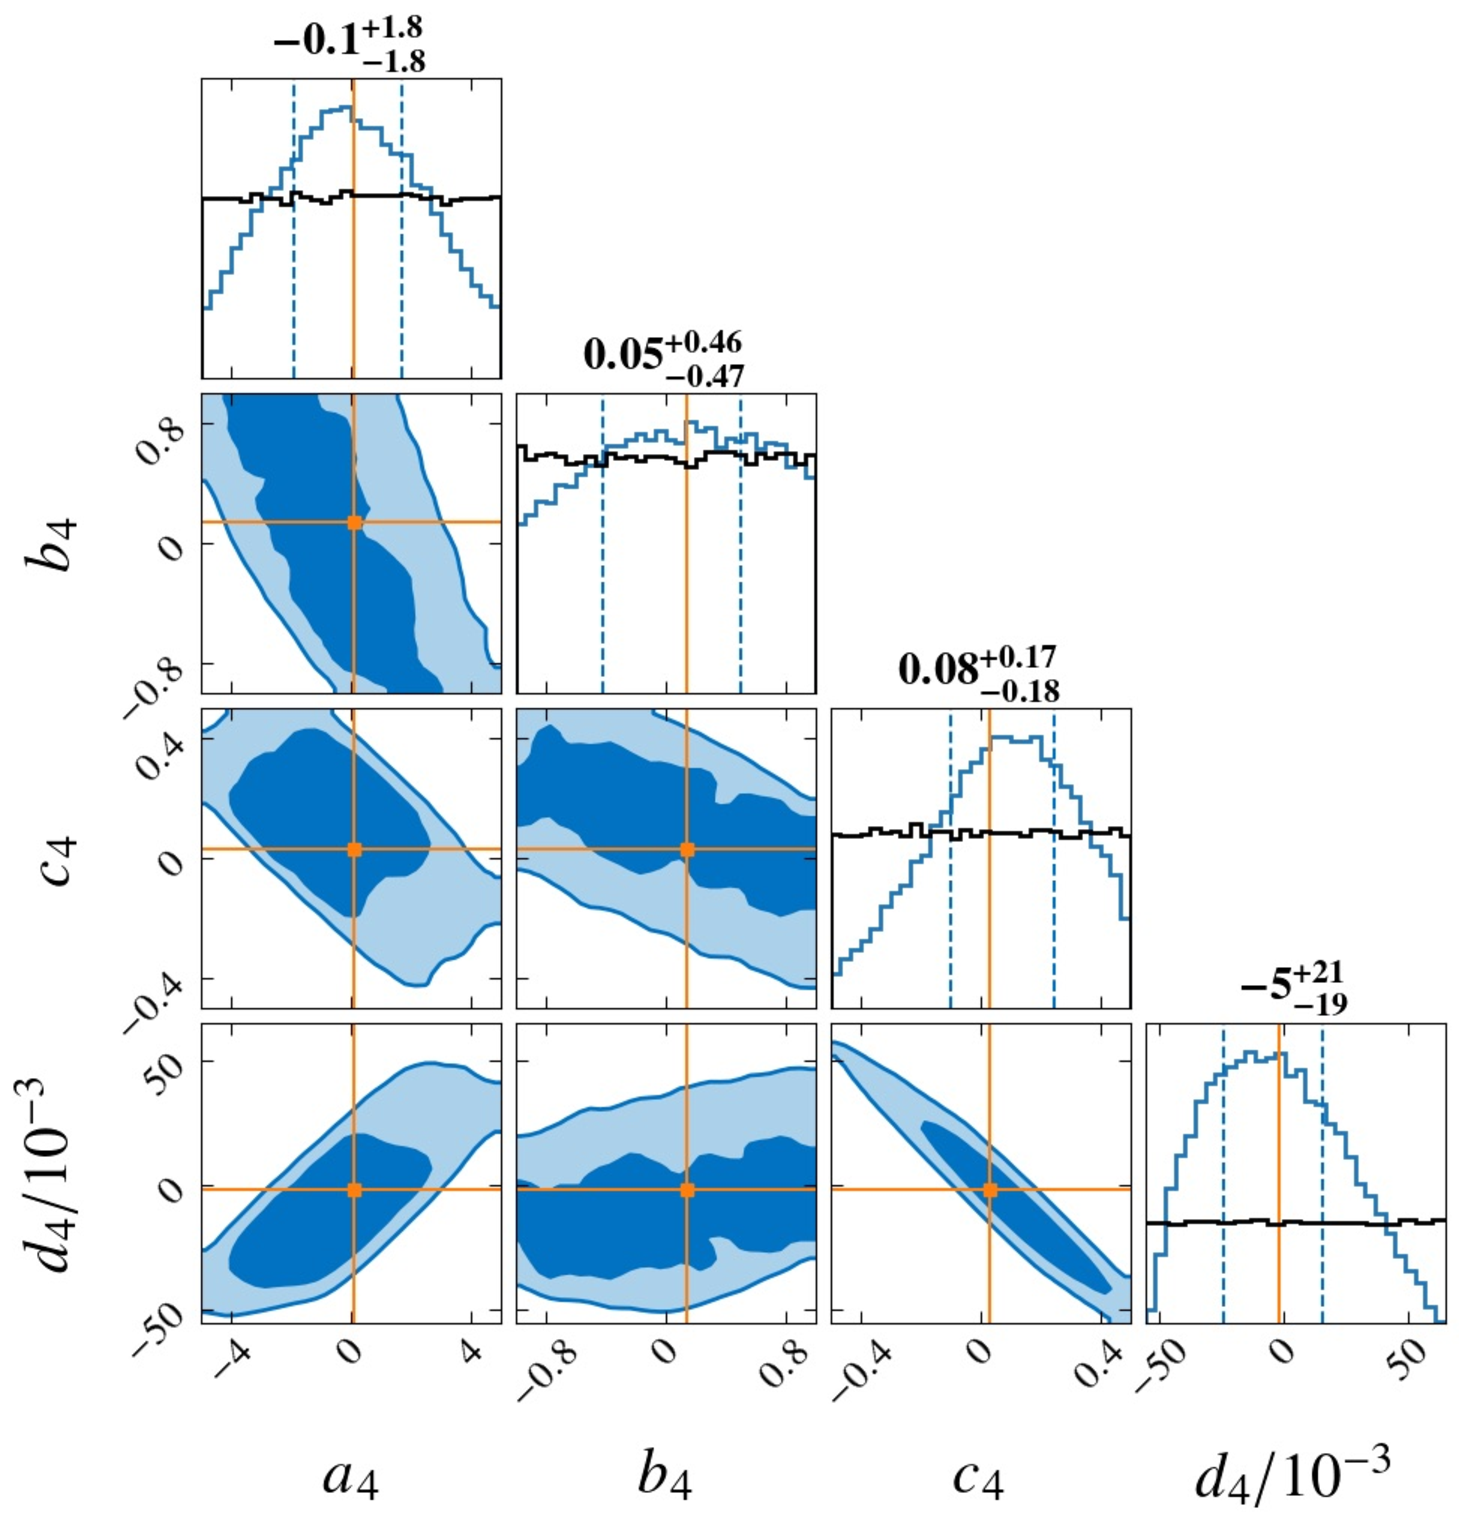
\includegraphics[width=0.8\linewidth]{Hyper_parameter_4d.pdf}
    \end{minipage}
    \vspace{3mm}
    \begin{minipage}[t]{\textwidth}
    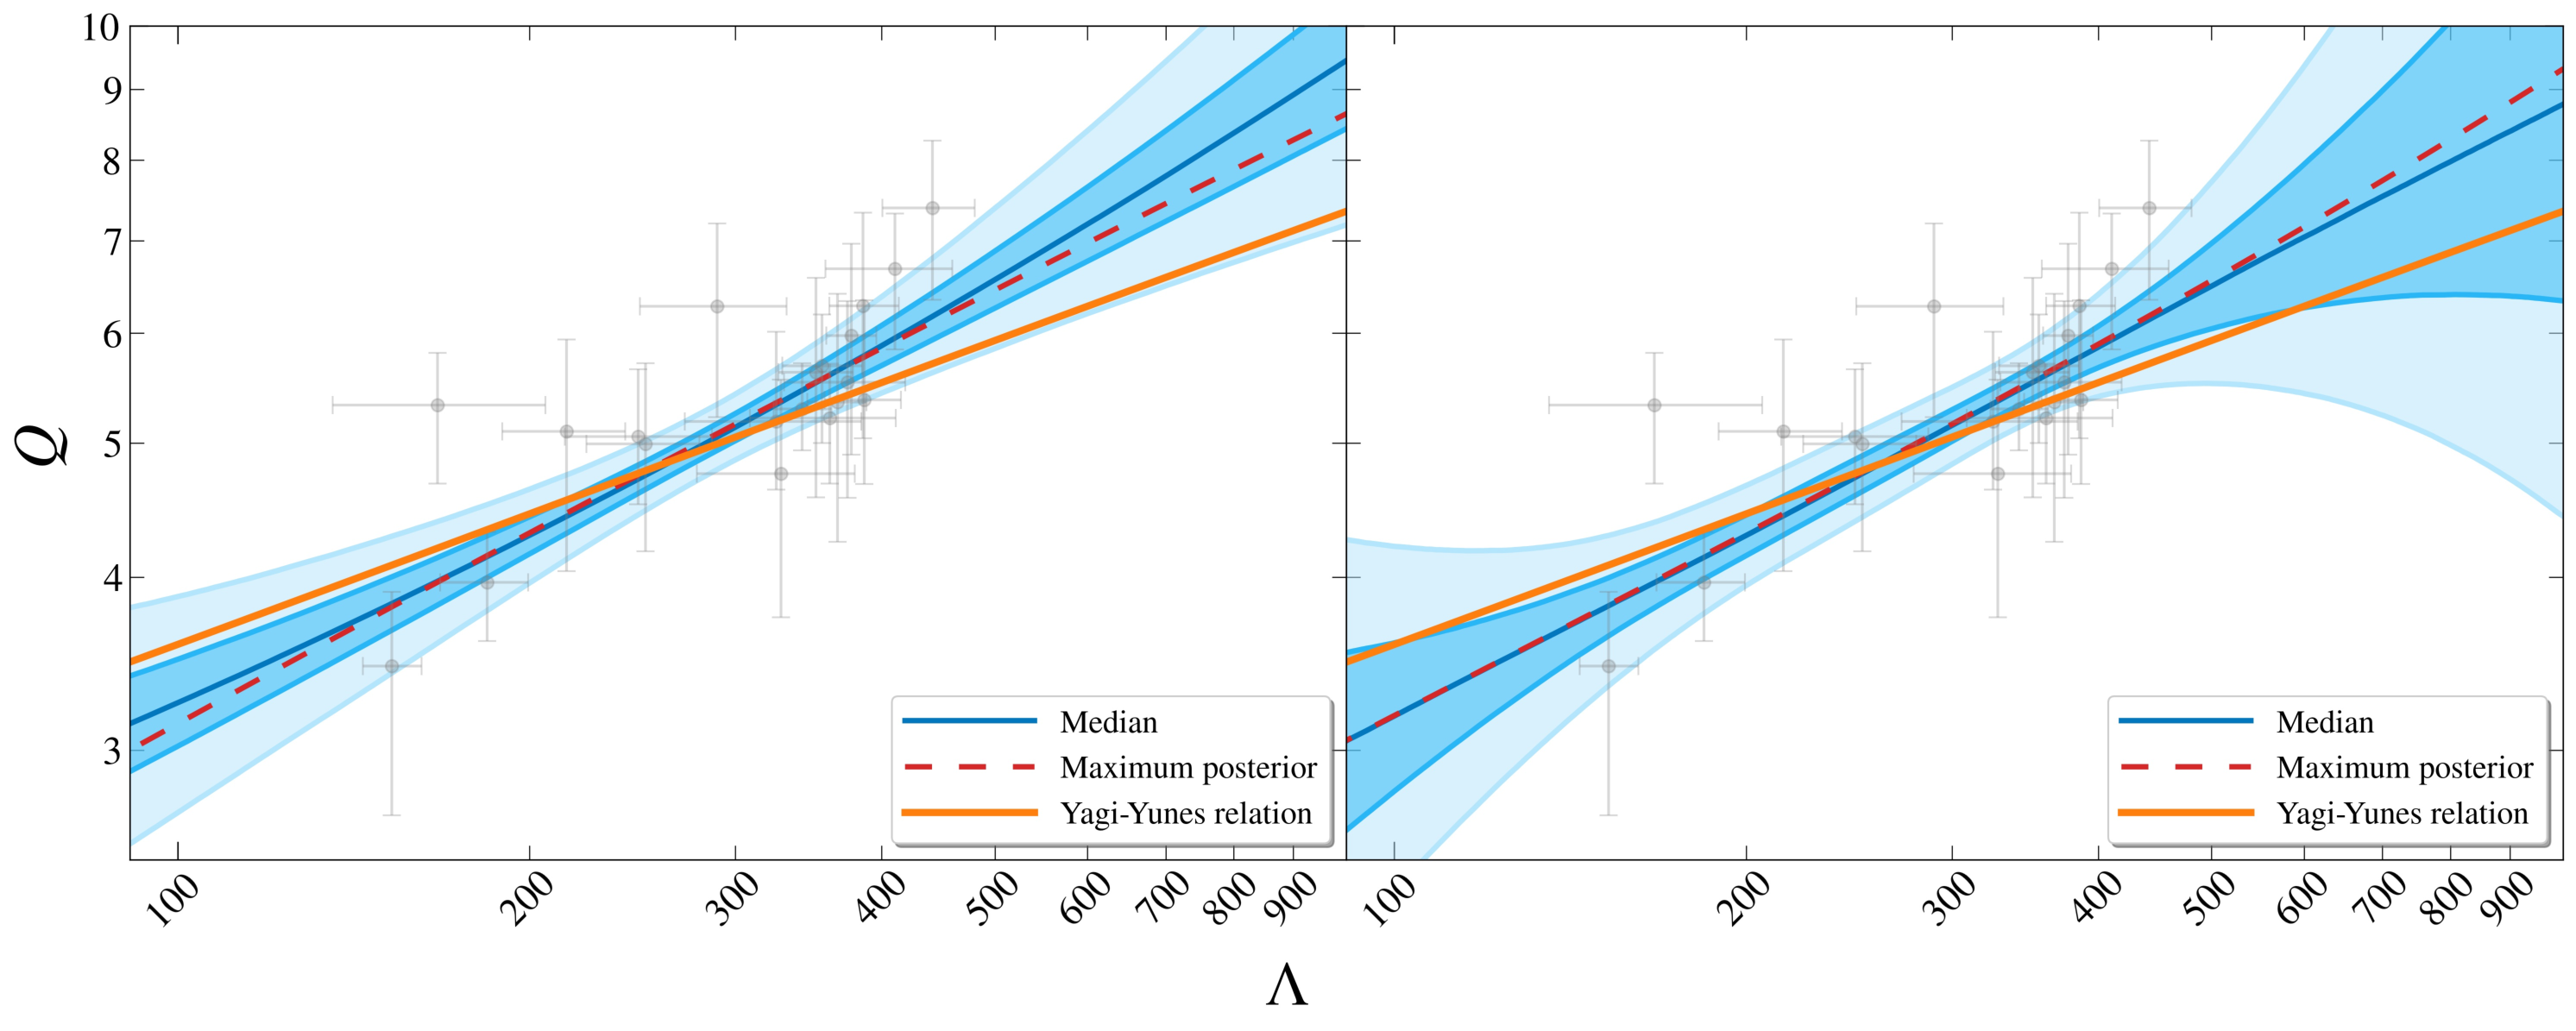
\includegraphics[width=\linewidth]{hierarchical_results_APR4_3d.pdf}
    \end{minipage}
    \caption{\label{3-d_4-d_Love_Q} Results of quadratic and cubic polynomial fitting models. The two upper panels demonstrate the posteriors of the hyperparameters. And the best fit values (see table~\ref{prior_table}) are marked in orange. The two bottom panels present the inference results in Love-Q plane, similar to figure~\ref{2-d_Love_Q}.
    }
\end{figure}
As shown in the previous two subsections, the observations from 20 simulated GW events can well constrain the two parameters in the linear model, while can not effectively constrain the five parameters in the quartic polynomial model. The two models are adopted in previous studies~\cite{Yagi:2013awa, Samajdar:2020xrd}, while here we further test the models in between them and see how the constraints change with the number of parameters. We perform the inference for the quadratic and cubic polynomial models, which contain three parameters $\{a_3, b_3, c_3\}$ and four parameters $\{a_4, b_4, c_4, d_4\}$, respectively. Similar to the linear model, the reference values of these parameters are obtained by directly fitting the Yagi-Yunes Love-Q relation and listed in table~\ref{prior_table}. The priors of the
hyperparameters keep the same as their counterparts in the quartic polynomial model, which are also listed in table~\ref{prior_table}.

We summarize the posterior distributions of the hyperparameters in the top row of figure~\ref{3-d_4-d_Love_Q}. In the quadratic model, strong degeneracy arises among the three parameters. The posterior of $b_3$ is almost the same as its prior. For $a_3$ and $c_3$, though the posteriors are narrower than the priors, their marginal distributions have very wide and flat peaks. In the cubic model, strong degeneracy still exists between $c_4$ and $d_4$, and the posterior of $b_4$ is also similar to its prior. Usually, posterior with large correlations and prior-like marginal distributions indicates redundant parameters in the model. Therefore, we conclude that the linear model is accurate enough in constraining the Love-Q relation with XG GW observations. This is consistent with the argument in Ref.~\cite{Samajdar:2020xrd} based on qualitative analysis, and in this work we present a quantitative demonstration. 

Same as before, we plot recovered Love-Q relations in the lower panels of figure~\ref{3-d_4-d_Love_Q}. We find the widths of the 90\% credible regions around $\Lambda \sim 400$ are similar for all the four models. While for
$\Lambda$ away from this region ($\Lambda \lesssim 200$ or $\Lambda \gtrsim 500$), the widths increase with the number of parameters. This may be the result of both the increased model complexity and the lack of data points in these
regions. 

%=============================
\section{Testing Modified Gravity: Dynamical Chern-Simons Gravity}
\label{sec:dCS}
%=============================

\begin{figure}[htbp]
    \centering
    \begin{minipage}{0.48\linewidth}
        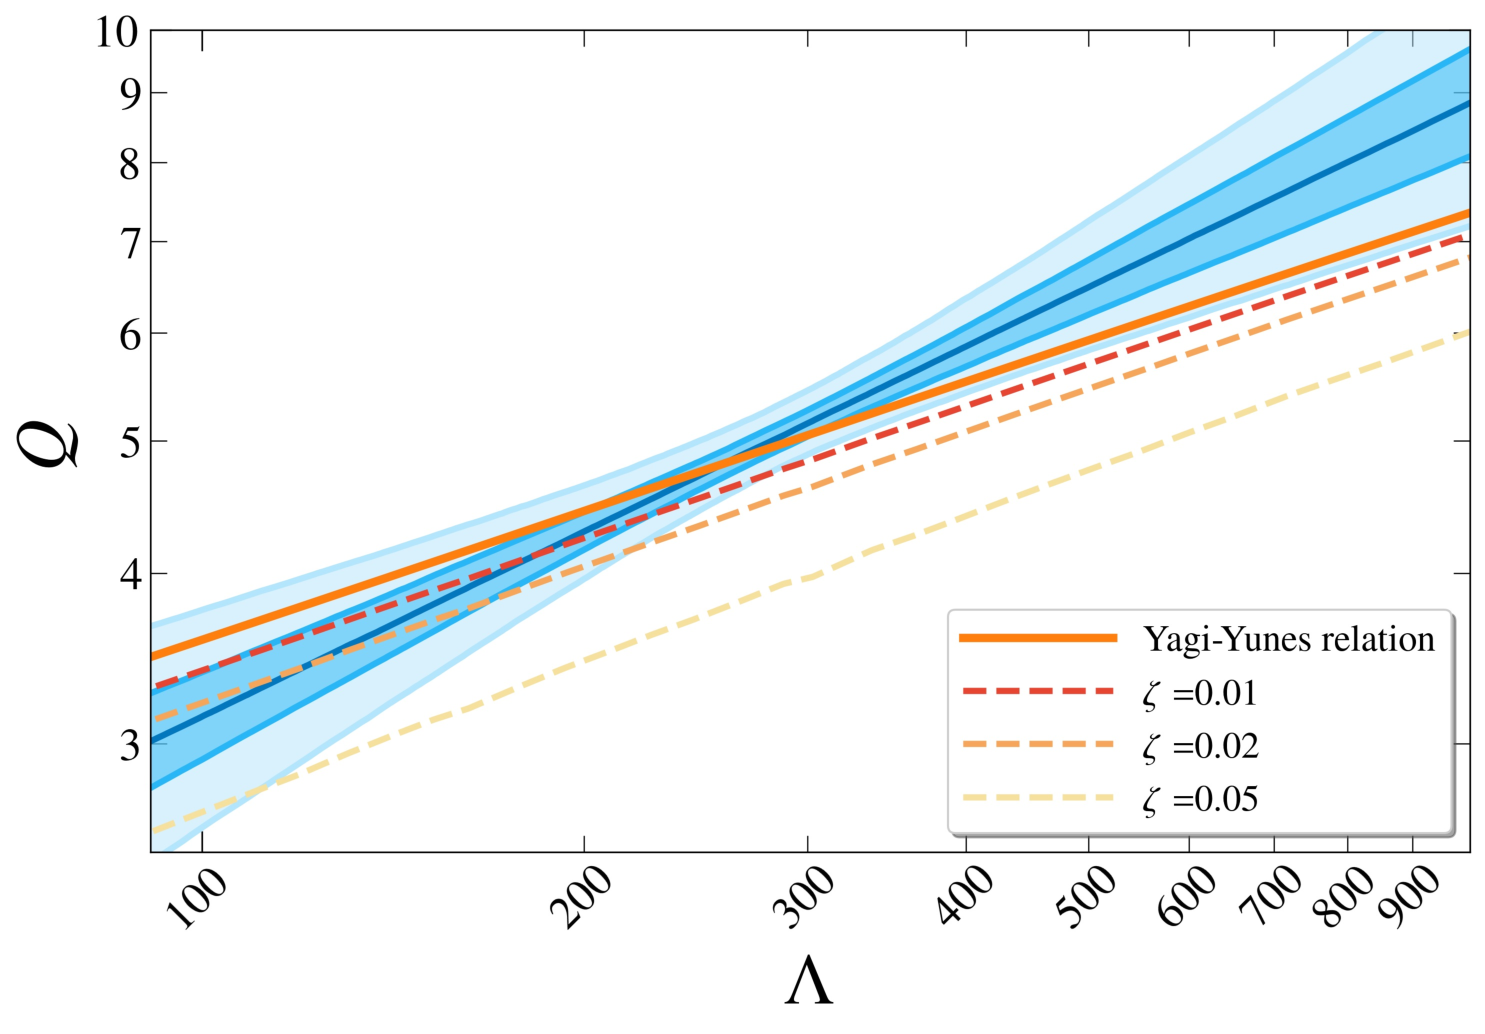
\includegraphics[width=\linewidth]{CS_zeta_APR4_2d.pdf}
    \end{minipage}
    \hfill
    \begin{minipage}{0.48\linewidth}
        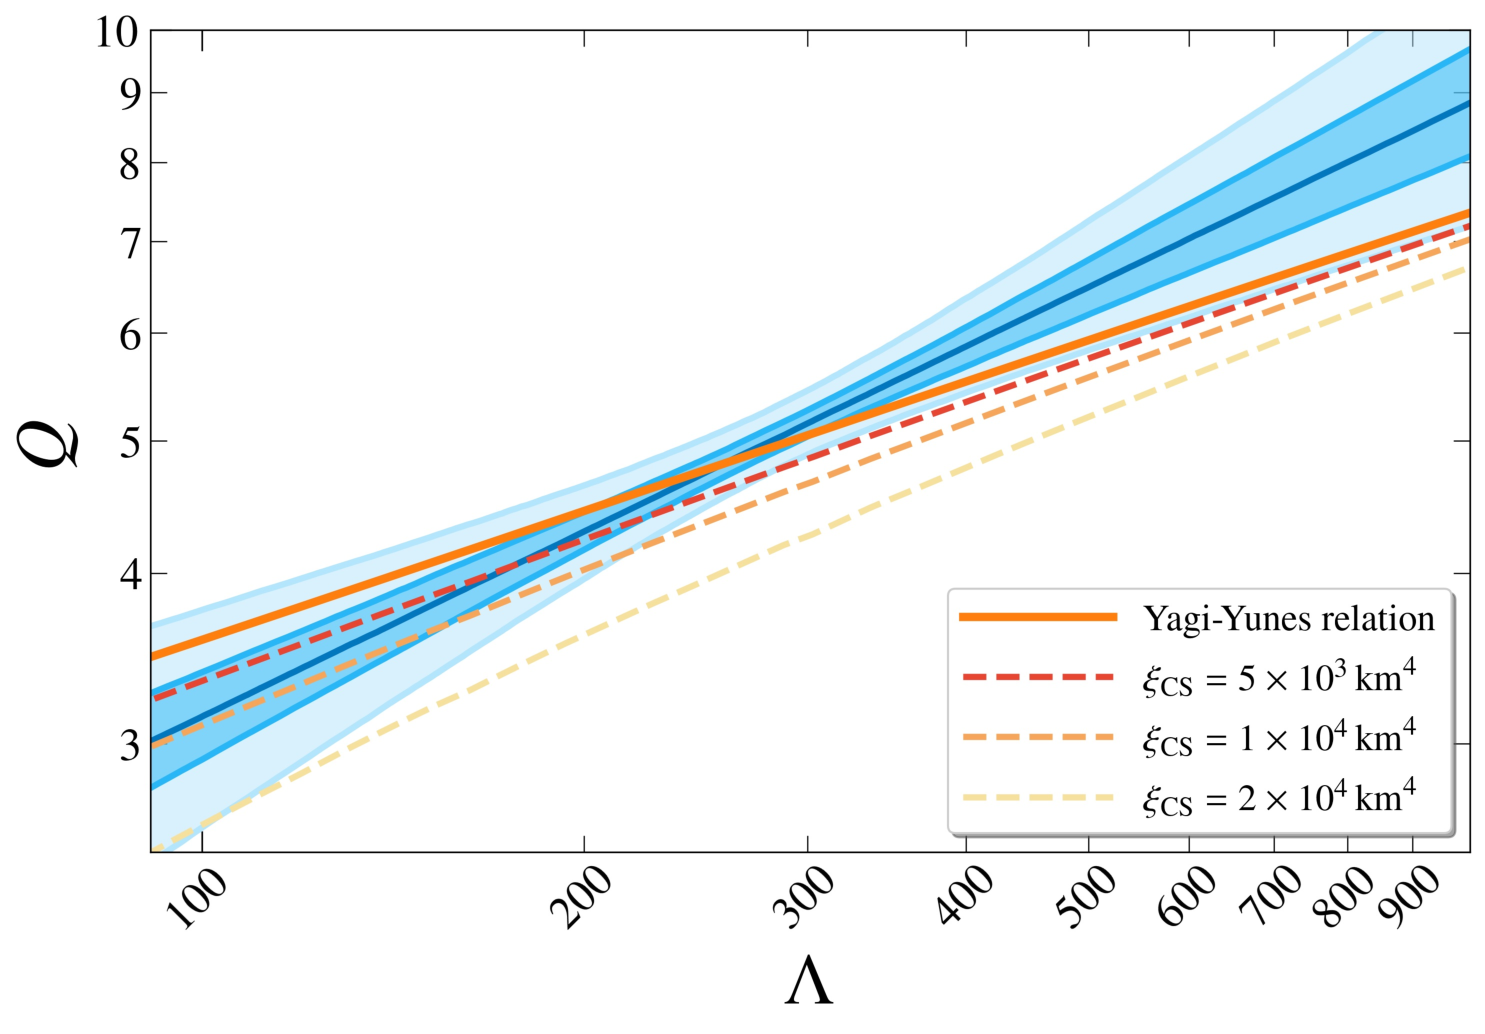
\includegraphics[width=\linewidth]{CS_xi_cs_APR4_2d.pdf}
    \end{minipage}
    \vspace{3mm}
    \begin{minipage}{0.48\linewidth}
        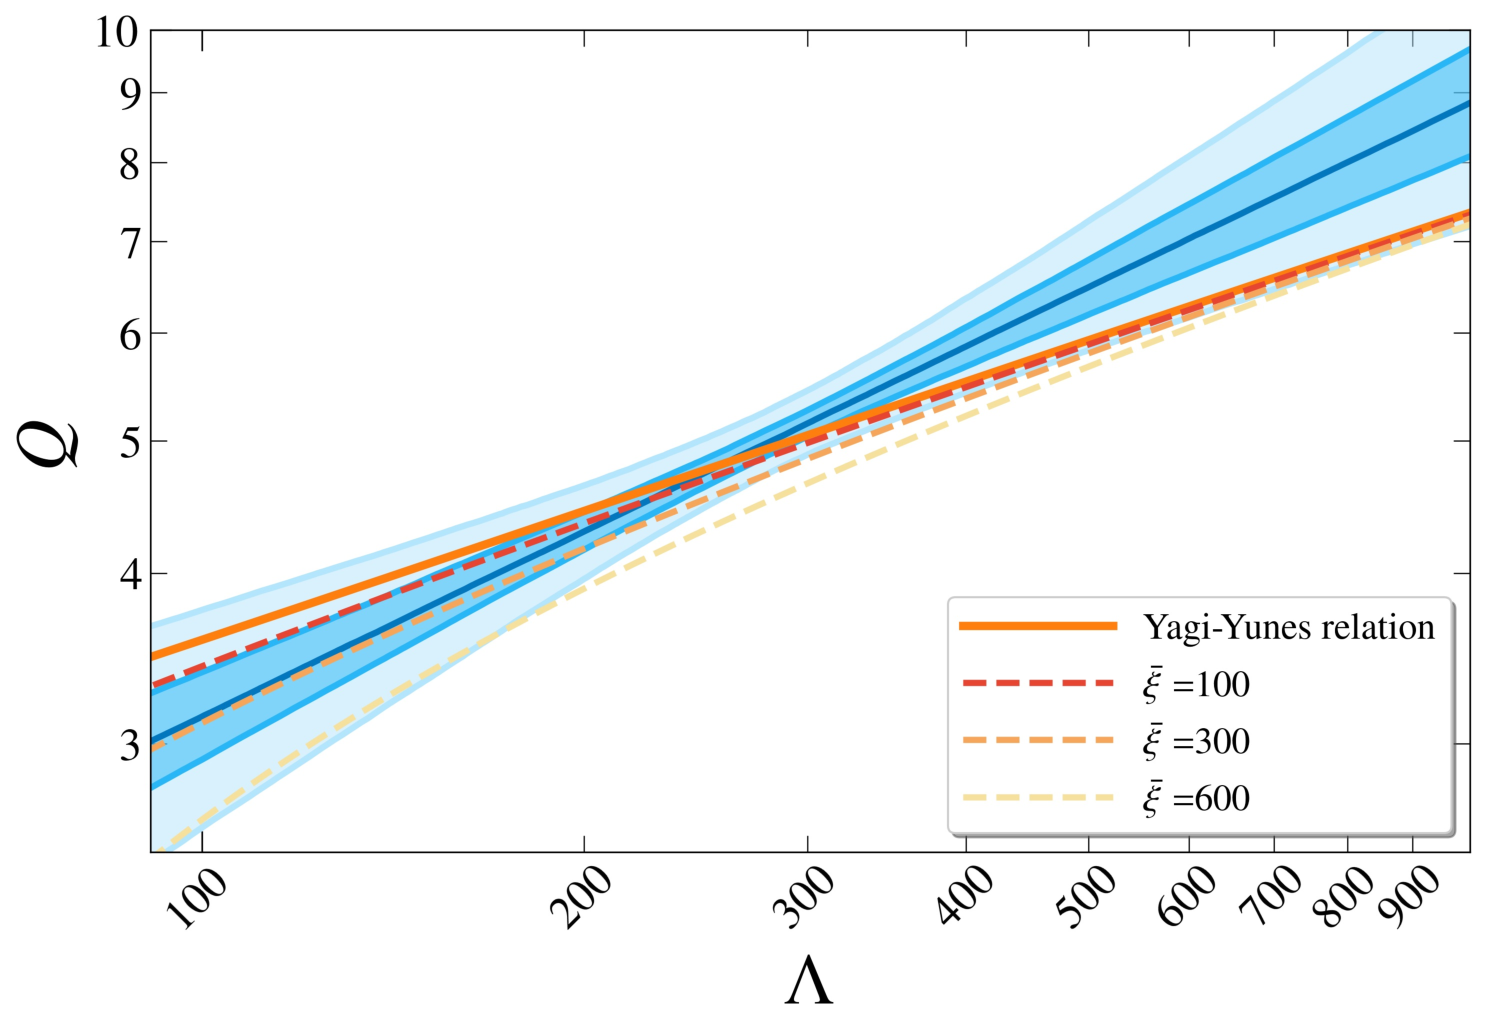
\includegraphics[width=\linewidth]{CS_xi_bar_APR4_2d.pdf}
    \end{minipage}
    \caption{Comparison of the hierarchical inference results and CS predictions with different coupling constants fixed. The blue regions are the same as figure~\ref{2-d_Love_Q} (Linear model). For each of the coupling constants of CS gravity $\zeta, \xi_{\mathrm{CS}}$ and $\bar\xi$, three possible values are taken and the corresponding Love-Q relations for APR4 EOS are drawn respectively as references.}
    \label{cs_Love_Q}
\end{figure}
In this section, we investigate the potential of testing gravity theories with the inferred Love-Q relation from the GW observations. The I-Love-Q test can be powerful when significant difference in I-Love-Q relation between GR and modified gravity theories exists, for example, some parity-violating theories~\cite{Yagi_2017, Yunes:2025xwp}. Here we take the dynamical Chern-Simons (dCS) gravity~\cite{Jackiw:2003pm, Smith:2007jm,Alexander:2009tp} for discussion, which is well-motivated from heterotic superstring theory~\cite{Polchinski:1998rq,Polchinski:1998rr}, loop quantum gravity~\cite{Alexander:2004xd,Taveras:2008yf,Calcagni:2009xz} and effective field theories of inflation~\cite{Weinberg:2008hq}. The dCS gravity introduces parity violation and quadratic curvature terms into the action~\cite{Alexander:2009tp,Gupta:2017vsl}
\begin{equation}
   \label{cs_action}
   S = \int \mathrm{d}^4 x \sqrt{-g}\left[ \kappa_g \mathcal{R} + \frac{\alpha}{4} \mathcal{\vartheta} \mathcal{R}_{\nu\mu\rho\sigma} {}^{*}\mathcal{R}^{\mu\nu\rho\sigma} - \frac{\beta}{2}\left(\nabla_{\mu}\mathcal{\vartheta}\nabla^{\mu}\mathcal{\vartheta}+2V(\mathcal{\vartheta})\right) + \mathcal{L}_{\mathrm{mat}}\right]\,,
\end{equation}
where $g$ is the determinant of the metric, $\kappa_g= 1/16\pi$, $\mathcal{R}$ is the Ricci scalar, $\mathcal{L}_{\mathrm{mat}}$ is the matter Lagrangian density and $\alpha$ and $\beta$ are the coupling constants in dCS gravity. The dual of the Riemann tensor is defined by 
\begin{equation}
    \label{dual riemann tensor}
    {}^{*}\mathcal{R}^{\mu\nu\rho\sigma}\equiv\frac{1}{2}\varepsilon^{\rho\sigma\alpha\beta}\mathcal{R}^{\mu\nu}{}_{\alpha\beta}
\end{equation}
where $\varepsilon^{\rho\sigma\alpha\beta}$ is the Levi-Civita tensor. We omit the potential for the pseudo-scalar field $\mathcal{\vartheta}$ in the action, following Ref.~\cite{Gupta:2017vsl}. $\mathcal{\vartheta}$ is taken to be dimensionless, making the quantity $\xi_{\mathrm{CS}}^{1/4} \equiv [\alpha^2/(\kappa\beta)]^{1/4}$ have a unit of $(\text{length})^{1}$ and can be explained as the characteristic length of dCS gravity~\cite{Yunes:2009hc,Yagi:2012ya}. 

%\ZW{Maybe you need to re-introduce the parameters in the Love-Q relation and the relation between them and the coupling constant in dCS gravity.}
The dCS gravity predicts Love-Q relations that are degenerate with the one in GR only when the coupling constants infinitely approach zero~\cite{Yagi:2013bca,Yagi:2013awa,Gupta:2017vsl}. The characteristic length has been constrained by current Solar System observations to $\xi_{\mathrm{CS}}^{1/4}<\mathcal{O}(10^8)$km~\cite{Ali-Haimoud:2011zme,Yagi:2012ya}. For a Love-Q test, Ref.~\cite{Yagi:2013mbt} obtained the dCS correction to the NS quadrupole moment and Ref.~\cite{Yagi:2011xp} indicates that the tidal deformability is the same as the one in GR at leading order in small coupling approximation $\zeta \equiv \xi_{\mathrm{CS}} M^2/R^6 \ll 1$, regarding the dCS gravity as an effective theory. Refs.~\cite{Yagi_2017,Yagi:2013mbt,Gupta:2017vsl} have discussed the Love-Q relation under dCS gravity and find that the relation becomes EOS-sensative with $\xi_{\mathrm{CS}}$ or $\zeta$ fixed. However, but with $\bar{\xi}\equiv \xi_{\mathrm{CS}}/M^4$ fixed, the Love-Q relation remains universal and the EOS variation is of $\mathcal{O}(1\%)$. Ref.~\cite{Gupta:2017vsl} parameterized the relation between the dCS correction to $Q$ (denoted as $Q_{\mathrm{CS}}$) and the tidal deformability $\Lambda$ as follows
\begin{equation}
    \label{cs_Love_Q_eq}
    \ln (Q_{\mathrm{CS}}/\bar{\xi}) = a + b \ln \Lambda + c \ln^{2} \Lambda
\end{equation} 
where the fitting coefficients $a=-3.443, b=-0.550$ and $c=-0.023$. 

Following Ref.~\cite{Yagi_2017}, we calculate the dCS Love-Q relation with $\zeta, \xi_{\mathrm{CS}}$ and $\bar{\xi}$ fixed respectively assuming the APR4 EOS, which has been assumed in our simulation in section~\ref{sec:simulation}. The results are demonstrated in figure~\ref{cs_Love_Q}. We compare the hierarchical Bayesian inference constraint of the Love-Q relation using the linear model (figure~\ref{2-d_Love_Q}) with some possible Love-Q relations with respect to certain coupling constants in dCS gravity. From figure~\ref{cs_Love_Q} we can conclude that our Love-Q test of dCS gravity can constrain the characteristic length $\xi_{\mathrm{CS}}^{1/4} \lesssim \mathcal{O}(10^1)$km, which is in agreement with the results given by Refs.~\cite{Yagi:2013bca,Yagi:2013awa}. For the other two coupling constants, our inference results place constraints of $\zeta \lesssim \mathcal{O}(10^{-2})$ and $\bar{\xi} \lesssim \mathcal{O}(10^{3})$.

%=============================
\section{Conclusion}
\label{sec:conclusion}
%=============================

In this work we adopted a hierarchical Bayesian framework to estimate the Love-Q relation of NSs. By separating the inferences of single-event parameters and hyperparameters, this framework provides a systematic and robust statistical method for hyperparameter estimation combining multiple GW events. We applied this framework to simulated GW events for a next-generation ground based GW detector network to examine the potential of constraining the Love-Q relation with GW observations. The results demonstrated that with this network, one can obtain a reliable measurement of the Love-Q relation through hierarchical Bayesian inference. We have also verified that the major information for inference of the hyperparameters is contained in the loudest 10 events, which is in agreement with the findings of Ref.~\cite{Lackey:2014fwa}.

We then investigated the impact of different parameterizations for Love-Q relation on the inference. We found that constraint of the Love-Q relation is insensitive to the parameterization in the region where most data points gather.
Also, as shown by the posterior distributions, degeneracies between hyperparameters exist in all cases studied. Furthermore, for all but the linear model, at least one hyperparameter was poorly constrained, exhibiting wide and flat posterior. These results indicate that a two-parameter (linear) model is sufficient for our data volume (20 GW events).

Finally, as a practical application, we compared our inference results with the theoretical predictions of the dCS gravity. The Love-Q relation measurement precision of our hierarchical Bayesian inference allows us to place a constraint on the dCS characteristic length $\xi_{\mathrm{CS}}^{1/4} \lesssim \mathcal{O}(10^1)$km. This result is consistent with previous works~\cite{Yagi:2013bca,Yagi:2013awa} and highlights the power of the Love-Q relation inference for testing gravity theories.

However, several issues remain to be addressed in future works. First, we have only considered the statistical uncertainties in our analysis, while systematic biases may arise from the inaccurate waveform model and the neglected spin precession effects. These biases can affect the inference results especially for high-SNR GW events from future ground based GW detections~\cite{Williamson:2017evr,Purrer:2019jcp,Gamba:2020wgg}. Second, the possible overlap of GW signals due to the high detection rate also leads to non-negligible biases in the measurements of GW parameters~\cite{Pizzati:2021apa,Hu:2022bji,Wang:2023ldq}. Plus, we have not taken account of the effect of the octupole or higher-order multipole moments of NSs, which enter the GW waveform as well and can be universally related to the quadrupole moment~\cite{Yagi_2017,Abac:2023ujg}. We leave a simultaneous inference of the universal relations between the tidal deformability, quadrupole and octupole moments to future works. Moreover, the universal relations we talk about are typically derived for a single NS. For BNS systems, universal relations may hold when the two NSs have similar masses, but whether they still hold for NSs with very different masses needs further inspections~\cite{Shao:2022koz}. Ref.~\cite{Saffer:2021gak} have made a first attempt to study this question, but a more thorough analysis is necessary. These extensions are left for future work and to sum up, future GW observations do have a promising prospect to infer the Love-Q relation and provide tests of gravitational theories. 


%=============================
\acknowledgments

\clearpage

\bibliographystyle{JHEP}
% \bibliographystyle{unsrt}
\bibliography{HBAGW_jcap}
\end{document}
